\documentclass[12pt]{ucthesis}
%I removed natbib, deluxe table, bibsetup,lscape,
\usepackage{aasmacros,algorithm, algorithmic, amsmath, amsfonts,amssymb,amsthm,array,color,enumerate,epsfig,graphicx,longtable,multirow,psfrag}
\usepackage[pagebackref=true]{hyperref}
% \usepackage[font=normal,justification=raggedright,singlelinecheck=false]{caption}
\usepackage[caption=false,font=normal,justification=raggedright,singlelinecheck=false]{subfig}
\usepackage{fixltx2e}

\makeatletter
\@ifundefined{showcaptionsetup}{}{%
 \PassOptionsToPackage{caption=false}{subfig}}
\makeatother


\usepackage{longtable}
\usepackage{wrapfig}
\usepackage{calc}

%\usepackage{titlesec}
%\titlespacing*{\chapter}{0pt}{-50pt}{20pt}
%\titleformat{\chapter}[display]{\normalfont\huge\bfseries}{\chaptertitlename\ \thechapter}{20pt}{\Huge}
%\citestyle{aa}
\bibliographystyle{plain}
%% below needs to be after biliographystyle to make bib single-spaced
\usepackage{tweak_ucthesis}
\usepackage{todonotes}
\usepackage{amsthm}
\usepackage{listings}
% \usepackage{wrapfig}
% \usepackage{subfigure}				
\newcommand{\R}{\mathbb{R}}


\newtheorem{defn}{Definition}[section]
% \newtheorem{prop}{Proposition}[section]
\newtheorem{rem}{Remark}[section]
\newtheorem*{note}{Note}


\input{adjoint-commands}
%\nofiles %% Uncomment for final edit of thesis.lof and thesis.lot

%% kluge to denote abstracts within thesis chapters
%\newcommand{\chabstract}{\medskip \bigskip {\bf \Large \centerline{Abstract} \bigskip}}
%% kluge to denote acknowledgements within thesis chapters
%\newcommand{\chacknowledgements}{\medskip \bigskip {\bf \Large \noindent Acknowledgements \bigskip \nopagebreak}}
%% kluge to fix figure/table numbers
%\renewcommand{\thefigure}{\thechapter.\arabic{figure}}
%\renewcommand{\thetable}{\thechapter.\arabic{table}}

%new command for theorems and all, the last bracket means to number within each chapter only
\newtheorem{remark}{Remark}[chapter]
%\renewcommand{\theremark}{\thechapter.\arabic{remark}}[chapter]
\newtheorem{prop}{Proposition}[chapter]
%\renewcommand{\theprop}{\thechapter.\arabic{prop}}
\newtheorem{definition}{Definition}[chapter]
%\renewcommand{\thedefinition}{\thechapter.\arabic{definition}}
\newtheorem{condition}{Condition}[chapter]
%\renewcommand{\thecondition}{\thechapter.\arabic{condition}}
\newtheorem{theorem}{Theorem}[chapter]
%\renewcommand{\thetheorem}{\thechapter.\arabic{theorem}}
\newtheorem{lem}{Lemma}[chapter]
\newtheorem{cor}{Corollary}[chapter]
\newtheorem{assumption}{Assumption}[chapter]
%\renewcommand{\thelemma}{\thechapter.\arabic{lemma}}

\let\originalleft\left
\let\originalright\right
\renewcommand{\left}{\mathopen{}\mathclose\bgroup\originalleft}
\renewcommand{\right}{\aftergroup\egroup\originalright}

%% if want to only compile parts
%\includeonly{frontmatter}
% \includeonly{distributed}
% \includeonly{security}
%~~~~~~~~~~~~~~~~~~~~~~~~~~~~~~~~~~~~~~~~~~~~~~~~~~~~~~~~~~~~~~~~~~~~~~~~~~~~~
\begin{document}
%~~~~~~~~~~~~~~~~~~~~~~~~~~~~~~~~~~~~~~~~~~~~~~~~~~~~~~~~~~~~~~~~~~~~~~~~~~~~~
%% declarations for front matter
\title{Optimization of Networked Dynamical Systems with Applications to Decentralized Freeway Control and Security of Traffic Systems}

%% go to bear facts to find your 'real' name
\author{Jack Daniel Reilly}

%% year you are getting this
\degreesemester{Fall}
\degreeyear{2014}

%% type of degree
\degree{Doctor of Philosophy}

%% committee chair
\chair{Professor Alexandre M. Bayen}

%% other committee members
\othermembers{
Professor Roberto Horowitz \\
Professor Scott Moura
}

%% total number of signers
\numberofmembers{3}

%% previous degrees (no longer needed, but need to designate as empty field)
\prevdegrees{}

%% main department
\field{Engineering -- Civil and Environmental Engineering}

%% campus
\campus{Berkeley}

%% make the title pages
\maketitle

%% copyright if you desire
\copyrightpage
\listoftodos

%% abstract
\begin{abstract}
This dissertation develops a general, scalable framework for controlling dynamical, networked systems based on mathematical optimization theory, with a strong focus on applications to freeway traffic management. The generality of the framework allows for controllers to consider arbitrary high-level objectives applied to systems with complex, nonlinear dynamics.

The dissertation presents a continuous freeway traffic model and its discretization developed specifically for onramp metering control, the application serving as the motivating example behind the theory developed subsequently. To apply effective control on such systems, a discrete-adjoint-based model-predictive-control (MPC) approach for controlling networked systems of conservation laws is presented, with explicit derivations for ramp metering applications. Linear scalability of the method with respect to network size and time horizon is derived for the discrete adjoint computations. To enable a more asynchronous control architecture, the dissertation presents a distributed optimization algorithm for dynamical, networked systems. The algorithm allows for a physical network to be partitioned into subnetworks that optimize locally and communicate only with adjacent subnetworks to achieve a globally optimal performance. 

Within the context of the \emph{Connected Corridors} project associated with UC Berkeley PATH, the developed theory was implemented in a production-level traffic management and simulation environment. Numerical examples using realistic, calibrated freeway networks are presented alongside the theory to motivate the highly practical aspects of the work. Simulations demonstrate the superiority of the MPC approach over existing methods widely used in practice.

The presented optimization tools are applied to an investigation of the security and vulnerabilities of traffic control systems. The potential impact of a compromise of freeway traffic metering lights is analyzed using MPC and multi-objective optimization tools. Several realizable scenarios that exploit traffic system vulnerability locations are constructed and simulated to illustrate the severity of compromises.

Investigations are made into optimal rerouting strategies while controlling only a subset of network flow. A novel behavioral model is developed to account for the interaction of controllable and uncontrollable agents sharing a single flow network, where latency is a function of total flow. Using static freeway traffic models and communication network models, a framework based on convex optimization techniques is presented for computing rerouting policies, with numerical results.

% effective management of transportation systems is crucial to supporting increasing vehicle demand into the future.

% To improve further the scalability of the adjoint approach and


% A taxonomy of potential attack vectors is developed to classify the cost and controllability of different the different attacks, among other features. 

% Explicit derivations of the approach are given for ramp metering applications along with numerical simulations on realistic freeway models to demonstrate the superiority of the MPC approach over existing methods widely used in practice.

% The splitting technique utilizes an asynchronous extension of the alternating direction method of multipliers algorithm that permits subproblems to apply the previously-developed discrete adjoint method.
\end{abstract}

%% begining of the front matter
\begin{frontmatter}
\renewcommand{\thepage}{\roman{page}}
\setcounter{page}{1}

%% dedication
\begin{dedication}
\null\vfil
{\large
\begin{center}
To Mamma Bear and Papa Bear
\end{center}}
\null\vfil
\end{dedication}

%% TABLE OF CONTENTS
\tableofcontents
\listoffigures
\listoftables

%% if you want a 'list of code' when using the code/sty file, include these
%% %\listofcodes
%% %\addcontentsline{toc}{chapter}{List of Code Examples}
%% %

%% acknowledgements
\begin{acknowledgements}
% -*- root: thesis.tex -*-
I would first like to thank Professor Alexandre Bayen for inviting me into his lab five years ago and for working closely with me during the entirety of that time. From him I learned much about rigor, thoroughness, persuasiveness, leadership and professionalism: traits which I have found to be the most valuable assets gained during my PhD. I am forever grateful for his patience and guidance.

I would also like to thank Professor Roberto Horowitz, Dr. Gabriel Gomes, and the other researchers in Professor Horowitz's lab. My work has benefited greatly from the different approaches to research and traffic in which I have participated. The discussions on real-world considerations such as queue-size limitations has enhanced the practicality of my research.

I give my gratitude to Professor Scott Moura, Professor Alexander Skabardonis, Professor Eli Yablonovitch, and Professor Steven Glaser for their guidance during my qualifying examination. Their feedback was valuable in directing the remainder of my research.
% I would like to also thank Professor Laurent El Ghaoui for suggesting I explore distributed optimization techniques, which I found to be fascinating and fruitful in traffic applications.

One of the most productive and enjoyable periods during my PhD was spent at the INRIA research center in Nice, France during Fall 2012, working with Dr. Paola Goatin and her student Maria Laura Delle Monache. I gained much insight into traffic models in general and how to develop a combined ordinary differential equation and partial differential equation model of freeway traffic. Their knowledge and methodology (i.e. mandatory coffee breaks) have permanently affected me.

I would also like to thank Raphael Marinier and Mihai Stroe of Google Road Traffic for their mentorship during my internship in Zurich, Switzerland in Summer 2013. Raphael's expertise in data analysis and focus on concrete results are skills I admire and attempt to emulate. I very much enjoyed the plethora of interesting traffic-related problems they have and their open-mindedness towards their solutions.

I thank again Professor Steven Glaser and thank Professor Raja Sengupta for welcoming me into the Civil Systems program mere days before the start of my Masters. Their novel approach to civil engineering is what reinvigorated my interest in the area, and I still regard my rash decision to switch into the Systems program as the best decision I have made.

I have had the pleasure to collaborate with many different students during my time in Berkeley. Specifically, I was lucky enough to work closely with Samitha Samaranayake over the last five years on many different projects and in many different venues (Surtardja Dai, La Val's, Nice, Tahoe, Gilman...). Additionally, over a brief three months, I benefited greatly from the intelligence and philosophical musings of S\'{e}bastien Martin while working on freeway traffic security.

A distinguishing feature of my PhD was the opportunity to implement my research within production systems. I would like to thank Branko Kerkez and Mario Magliocco for their infinite patience with a greenhorn as I worked on the iShake project. I would also like to thank Joe Butler and many others, including Gabriel Gomes and Dimitris Triantafyllos, at CCIT and PATH for their dedication to supporting research in a professional environment and professionalism in a research environment.

To my dearest friends, Devon, Jack, Matty, Zack, Heidi, Timothy, Katelyn, thank you for embodying all that I find good in this world.

And finally and foremost, I give my thanks and love to my mother Joanne, father Jim, and my brothers and best friends Jimmy and Christopher.
\end{acknowledgements}

\clearpage

\end{frontmatter}

\chapter{Introduction}
\label{sec:introduction}

\section{Motivation}
\label{sec:motivation}

% \todo[inline]{lots of ``systems'' written here}

Modern infrastructure, particularly systems associated with public use such as freeway networks and water supplies, exist within a world with decreasing physical space and resources. For instance, freeways often cannot add additional lanes to accommodate increased demands. Thus, one must rely upon better management systems and control algorithms in order to maximize performance within the limitations of the existing system. These ``smart'' systems make use of sensing instrumentation to estimate real-time conditions and modeling of the underlying physical dynamics to predict and plan for future states.

The focus of this thesis is the development of methods for the advanced modeling and control of such networked dynamical systems. The goal is to provide operational managers with scalable, flexible, and robust algorithms that can leverage the well-instrumented and highly-connected control infrastructure present on modern systems. 

The remainder of this section discusses the \emph{Connected Corridors} project (Section~\ref{sec:connected-corridors}) on \emph{integrated corridor management} (ICM), which served as the context in which this work was conducted, followed by an overview of \emph{model predictive control} (MPC) methods and their suitability in solving some of the main objectives put forth in the \emph{Connected Corridors} project (Section~\ref{sec:model-predictive-control}). The section concludes with a summary of the original contributions presented in this thesis (Section~\ref{sec:contributions}).

\section{Connected Corridors}
\label{sec:connected-corridors}

\emph{Connected-Corridors} is a project funded by the California Department of Transportation with the goal of creating the next generation of traffic management tools~\cite{connected-corridors,miller2010san}. While most current systems consider the freeway networks as independent from the city-street \emph{arterial} road networks, \emph{Connected Corridors} is tasked with creating an integrated approach to traffic management (referred to as ICM) which accounts for their dual performance. The project has demonstrated innovative control and estimation approaches to ICM on macroscopic and microscopic simulation environments (presented in Section~\ref{sec:numerical-results-adjoint}), with the ultimate plan of transferring the knowledge to a physical test-site within California located near the I210 freeway.

The proposed ICM system possesses the following capabilities.

\begin{itemize}
	\item \textbf{Estimation}: Operators have access to a real-time estimation of the traffic state along the major freeways and adjacent arterials~\cite{work2010traffic,Jacqueta,eisenman2006number}.
	\item \textbf{Simulation}: Well-calibrated and efficient traffic models allow operators to simulate many different future traffic conditions~\cite{Muralidharan2009b,dervisoglu2014macroscopic,Hunter}.
	\item \textbf{Control}: Traffic signal and message sign plans are computed online for a variety of specialized objectives and serve as an optimized decision support tool~\cite{Reilly2013b,Reilly2014b}.
\end{itemize}

Control schemes implemented by the system include coordinated traffic light metering plans on freeway onramps (commonly referred as ramp metering, see Section~\ref{sec:continous-and-discrete-traffic-model-for-ramp-metering}) and traffic flow diversion around incidents via changeable message signs~\cite{Samaranayake2014}. 

\begin{figure}[htbp]
	\centering
	\includegraphics[width=0.7\textwidth]{diagrams/f2}
	\caption[\emph{Connected Corridors} control system architecture.]{The freeway state estimation, prediction and calibration submodules enable an MPC-based framework that computes coordinated, predictive decision-support strategies for numerous applications. Limited customization is required to extend the adjoint-based MPC controller to specific objectives or actuation types.}
	\label{fig:decision-support}
\end{figure}

To satisfy the above requirements, \emph{Connected Corridors} focuses on a number of submodules which are developed independently, but composed in a variety of ways to create high-level, comprehensive support tools. Figure~\ref{fig:decision-support} shows several of the developed submodules and how they can be composed to create an MPC controller (explained in Section~\ref{sec:model-predictive-control}). Subsequently, the controller submodule is leveraged by a number of actuation strategies which have similar architectural requirements. For instance, both ramp metering and dynamic rerouting require real-time estimation and a calibrated freeway model to compute effective control strategies. Via submodule composition, much of the technology can be reused between the applications. This work contains the theory and implementation of constructing such controller submodules which efficiently exploit the structure of freeway networks.

\section{Model Predictive Control}
\label{sec:model-predictive-control}

Central to the \emph{Connected Corridors} approach of freeway traffic decision support is the concept of \emph{model predictive control} (MPC)~\cite{Muralidharana,Donoghue2013Splitting,Frejo2011}. Generally speaking, MPC schemes successively compute a control policy which maximizes the performance, according to a provided criteria, of the system over the immediate future, where this work assumes the future to be of finite duration. The policy generated from the MPC scheme is recomputed as frequently as the real-time state estimation and computation times permit. Thus, associated with an MPC problem are two time periods: the \emph{update time} representing how often the MPC policy is recomputed online, and the \emph{time horizon} representing how far into the future for which the MPC policy will account. A more detailed treatment of MPC schemes is given in Section~\ref{sec:model-predictive-control-overview-adjoint-section}.

The requirements of an online MPC controller for a traffic system are depicted in Figure~\ref{fig:decision-support}. At the base of the method is a mathematical model of the physical system, referred to as the \emph{forward system}. These models often require calibration using historical sensor measurements to set the model parameters. To fully specify the simulation, an \emph{initial condition} is specified (i.e. estimation), as well as the \emph{boundary conditions} at the exteriors of the system over the entire time horizon of the MPC problem (i.e. prediction). All these requirements are satisfied by components within the \emph{Connected Corridors} system~\cite{Muralidharan2009b,dervisoglu2014macroscopic,work2010traffic}, making MPC control a natural fit for research and development in the project.

The focus of this thesis is the efficient and flexible design of MPC optimization techniques and their applications to freeway control systems. At the heart of the developed approach is the \emph{discrete adjoint} method for gradient computations within first-order gradient descent methods (Chapter~\ref{chapter:adjoint}). The efficiency of the developed method enables \emph{online} application of MPC to the control of large freeway networks (on the order of tens of miles) with frequent recomputations (on the order of one minute) to ``close the loop'' with real-time measurements.

In addition to the well-established ramp metering control infrastructure, the emergence of smartphones and connected vehicles and crowd-sourcing data collection~\cite{Reilly2013,Ervasti2011,dashti2013evaluating} has made mass rerouting strategies a new, viable form of control. This thesis showcases this potential by including an investigation of rerouting strategies for a subset of flow on networks. Inspired by the increasing penetration of navigation devices in vehicles (e.g. dedicated units, smartphone applications), a single navigation provider may advise a signification portion of the total flow on some networks, thus potentially affecting traffic conditions based on their advice. This potential can be harnessed to reduce the inefficiencies of \emph{selfish routing}~\cite{roughgarden2002bad,krichenetac} and drive network behavior towards \emph{socially optimal} conditions.

\section{Contributions}
\label{sec:contributions}

This thesis contains the following contributions to the problem of optimal control of networked dynamical systems, applied to the field of traffic control.

\begin{itemize}
	\item \textbf{A novel continuous freeway traffic model suitable for finite-horizon optimal control problems}~\cite{delle2014pde,Reilly2013b}.
	\begin{itemize}
		\item The model represents an extension of the networked \emph{Lighthill-Richards-Whitham} (LWR) PDE traffic model~\cite{lighthill1955kinematic,richards1956shock} proposed in~\cite{garavello2006traffic}, where onramps are modeled as ODE buffers to guarantee \emph{strong} boundary conditions and flow conservation at the network boundaries.
		\item A discretized version of the continuous model is derived for optimal control application using Godunov's method~\cite{godunov1959,lebacque1996godunov}.
	\end{itemize}
	\item \textbf{A method for optimal control of networked conservation law systems based on discrete adjoint calculations}~\cite{Reilly2013b,Samaranayake2014}.
	\begin{itemize}
		\item This work develops a framework for converting a continuous time and space control problem on a physical network, where edges behave according to a conservation law, into a discrete, finite-horizon optimal control problem using Godunov discretization.
		\item The application of the discrete adjoint method~\cite{Giles2000,Duffy2009,Apice2010Modeling,Gugat2005} to compute gradients for the above problem is presented, with an analysis of the linear scalability of the approach in discrete time and discrete space for sparse network structures.
		\item An explicit formulation of the discrete adjoint method is given for the application of coordinated ramp metering control~\cite{Papageorgiou1991,Frejo2011,Kotsialos2004,gomes2006optimal} for freeway networks.
		\item Simulations of MPC on a macroscopic model of the I15 South Freeway in San Diego, California demonstrate the practical nature and the robustness to measurement noise of the research.
	\end{itemize}
	\item \textbf{A decentralized algorithm and control infrastructure for networked dynamical systems}~\cite{Reilly2014b}.
	\begin{itemize}
		\item This thesis presents a new distributed optimization method based on the \emph{alternating directions methods of multipliers} (ADMM)~\cite{Boyd2010a,gabay1976dual,mota2012distributed} algorithm for solving  optimal control problems over subnetworks in parallel. The splitting method is done in such a way to only require communication between physically-neighboring subnetworks.
		\item Differing from similar work where subsystems only share control variables~\cite{mota2012distributed,camponogara2009distributed}, the presented method allows for subsystems to share both control \emph{and state} variables, an assumption necessary for the distributed control of traffic networks and hydrological systems.
		\item A discrete adjoint formulation is presented for efficient solution of subsystems with coupled control and state variables.
		\item An implementation of a distributed ramp metering and variable speed limit controller is simulated on a realistic macroscopic freeway network, demonstrating advantages over other proposed communicative controllers.
	\end{itemize}
	\item \textbf{An analysis of the security of traffic control systems and coordinated ramp metering attacks}~\cite{Reilly2014c}.
	\begin{itemize}
		\item A classification of traffic system vulnerability locations is constructed across such categories as cost of attack, effectiveness, and directness of control.
		\item A novel analysis of the potential damage and impact of coordinated ramp metering attacks is conducted using adjoint-based optimal control and multi-objective optimization tools.
		\item Illustrative attack scenarios are constructed and numerically investigated on realistic freeway networks. A web-based coordinated ramp metering attack tool was created to implement the interactive optimization approaches presented in the work~\cite{smartroadswebsite}.
	\end{itemize}
	\item \textbf{A framework for rerouting a subset of vehicles on freeway networks}.
	\begin{itemize}
		\item As opposed to standard system-optimal routing problems~\cite{ziliaskopoulos2000linear,Kelly} where all flow is controllable, we construct a network-flow optimization problem which allows one to specify a \emph{compliance rate} of cooperative vehicles. The proposed model captures the delays induced by the noncompliant vehicles.
		\item To account for the possibility of noncompliant drivers adapting to the new flow conditions, we propose a behavioral model, referred to as \emph{bounded tolerance}, which assumes that noncompliant drivers have bounded rationality and will only switch routes under significant increases in delay.
		\item Numerical examples for communication networks and freeway systems demonstrate the effectiveness of the method.  
	\end{itemize}
\end{itemize}

\section{Organization}
\label{sec:organization}

The rest of the article is organized as follows.

Chapter~\ref{chapter:freeway-network-model} presents the continuous and discrete freeway models which serves as the running application of the theory presented subsequently.  After covering preliminaries on networked PDE systems, the derivation of and motivation behind the model are given.

Chapter~\ref{chapter:adjoint} presents the discrete adjoint approach to optimal control of networked conservation laws. Presented first is a general overview of the discrete adjoint method, followed by its specific instantiation for discretized physical network systems. The application to coordinated ramp metering is then presented with numerical examples. The chapter concludes with the distributed, asynchronous formulation of the adjoint optimal control method via subnetwork splitting.

Chapter~\ref{chapter:security} presents a study of traffic control systems and their vulnerabilities. After defining the specific control system under consideration and its security weaknesses, the work gives an in-depth study of coordinated ramp metering attacks.

Finally, we conclude with a overview of the work presented, as well as directions for future research.

The material presented in Chapters~\ref{chapter:freeway-network-model} and~\ref{chapter:adjoint} was done collaboratively as part of the \emph{Optimal Reroute Strategies for Traffic Management} (ORESTE) project between UC Berkeley and INRIA research institute in Sophia-Antipolis, France. Chapter~\ref{chapter:security} also contains research stemming from collaborations with Sebastien Martin and Mathias Payer. Chapters~\ref{sec:distributed_optimization_of_coupled_dynamical_systems} and~\ref{chapter:le} contains research conducted independently.
\chapter{Freeway Network Model}
\label{chapter:freeway-network-model}

\section{Preliminaries of Networked Conservation Laws}

\subsection{Networked Conservation Laws}

\subsection{Riemann Solvers}

\subsection{Godunov Discretization}

\section{Continuous and Discrete Traffic Model for Ramp Metering}
\label{sec:continous-and-discrete-traffic-model-for-ramp-metering}

\subsection{Overview on Traffic Models and Ramp Metering}

\subsection{LWR Equation}

\subsection{Flow Conservation at Network Boundaries}

\subsection{Continuous PDE-ODE Freeway Model}

\subsection{Discrete Freeway Model}
\section{Continuous and Discrete Traffic Model for Freeway Control}
\label{sec:continous-and-discrete-traffic-model-for-ramp-metering}

In this section, we derive and motivate the continuous freeway network traffic model and discuss its improvements over existing models. We also present the discretized version of the continuous model, which is used extensively in applications in the remainder of the thesis. 

\subsection{LWR Equation}

The Lighthill-Whitham-Richard (LWR) equation~\cite{lighthill1955kinematic,richards1956shock} is a scalar conservation law used to represent the evolution of vehicle density on a section of linear roadway. The distinguishing assumptions in the LWR model deal with the flux function, $f\left(\rho\right)$, referred to as the \emph{fundamental diagram of traffic}. Namely, we assume the following rules on $f$:

\begin{enumerate}
	\item $f\left(\rho \right) = \rho v\left(\rho \right)$, where $v$ is the velocity of the vehicle density.
	\item $v\left(\rho \right)$ is a decreasing function of $\rho$.
	\item $f$ is defined over the values $\left[0,\rho^{\max}\right]$, where $\rho^{\max}$ is considered the \emph{jam} density.
	\item $f\left(0\right) = f\left(\rho^{\max}\right) = 0$.
\end{enumerate}

The four rules above fit well with our intuition of road traffic. Rules 1 and 2 state that the flux varies as the velocity varies, and that as the roadway gets more congested, the speed of the vehicles will only decrease. Rule 3 fits with the physical interpretation of vehicle as being non-negative, and that there must be an upper limit of vehicle density (due to minimum car lengths). Rule 4 states that no vehicles will have no flow, and that flow completely breaks down at the maximum density.

\begin{figure}[htbp]
	\centering
	\includegraphics[width=0.6\textwidth]{diagrams/fd}
	\caption{The Greenshields (quadratic) flux function is one example of a fundamental diagram.}
	\label{fig:greenshields-fd}
\end{figure}

An example of a quadratic fundamental diagram, known as the \emph{Greenshields} flux function, is given in Figure~\ref{fig:greenshields-fd}. The term \emph{critical density}, $\rho^{\text{cr}}$, is reserved for the density value where the maximum vehicle flux, $f^{\max}$, is obtained. The maximum flux can also be viewed as the \emph{capacity} of the road under consideration, where demand in excess of the maximum flux will lead to congestion and traffic jams.

\subsection{Continuous PDE-ODE Freeway Model}
\label{sec:continuous-pde-ode-freeway-model}

We concern ourselves with a \emph{linear} freeway section, meaning that we are only interested in one freeway mainline, with any number of onramps and offramps coming together at junctions. While the approach can be readily extended to mainline-to-mainline junctions, we exclude the analysis for the sake of presentation.

Thus, a freeway network can be viewed as a sequence of junctions, where each junction contains four links: an upstream mainline, a downstream mainline, an onramp and an offramp, as visualized in Figure~\ref{fig:simple-junction}. Note that a single mainline link (i.e. a stretch of mainline in between two junction points) will serve as the upstream mainline of one junction and the downstream mainline of the subsequent junction.

\begin{figure}[htbp]
	\centering
	\includegraphics[width=0.6\textwidth]{diagrams/simple-junction}
	\caption{A freeway junction consisting of an upstream mainline $I_1$, downstream mainline $I_2$, onramp $R_1$ and offramp $R_2$.}
	\label{fig:simple-junction}
\end{figure}

\subsubsection{Weak Boundary Conditions and Vehicle Conservation}

In reality, one cannot consider the evolution of a stretch of freeway in complete isolation with respect to its surrounding traffic network, as the dynamics are coupled at every junction point via Riemann solvers (Section~\ref{sec:riemann-solvers}). Thus, to account for the behavior at the extremities of the network, one must consider boundary conditions.

The standard approach to boundary conditions is to prescribe a time-varying density $\rho^0\left(t\right)$ at each extremity point of the network. Due to the concave shape of the fundamental diagram of traffic, density waves may propagate from within the system outwards to the network extremities, in both the upstream and downstream directions.

As an example, one could consider the behavior upstream of onramp $R_1$ as being the solution of a Riemann problem of the form in Equation~\eqref{eqn:riemann-problem}, where $\rho_-$ is the upstream boundary condition, and $\rho_+$ is the state within an onramp. Whenever $f\left(\rho_+\right)<f\left(\rho_-\right)$ and $\rho_+ > \rho^{\text{cr}}$, then it can be shown~\cite{lebacque1996godunov,garavello2006traffic} that the vehicle flux across the boundary is $f\left(\rho_+\right)$ and is thus insensitive to the value of $f\left(\rho_-\right)$. One can view this event as a \emph{loss of information} at the left boundary of the network, as the backward-moving congestion wave prevented information about the boundary condition from entering the network. Systems which possess this property are said to have \emph{weak boundary conditions}~\cite{strub2006weak}.

This property of traffic network modeling is undesirable in traffic management applications, as the flux of vehicles at network boundaries is dependent upon the state of the system, which in turn is dependent upon the control scheme being applied. Summarizing, different control schemes can lead to different vehicle demands, which is not a realistic assumption, can actually be exploited by control schemes. As the goal of the current traffic model is to be used in control applications, we develop an alternative approach which effectively turns the weak boundary conditions into \emph{strong} boundary conditions which guarantee vehicle flux conservation.

\subsubsection{Onramps as ODE Buffers}

Instead of modeling boundary conditions as vehicle densities, we consider a time-varying boundary \emph{flux}, $\demandsym\left(t\right)$ entering onramp $R_1$ and make the simplifying assumption that the offramp $R_2$ has infinite capacity and thus does not influence the evolution of the system\footnote{Motivation behind the offramp model is the focus on ramp-metering applications in this thesis, and the general lack of available sensor data on freeway offramps, making accurate modeling of offramp state difficult.}.

The onramp $R_1$ stores the boundary flux in a vehicle \emph{buffer} modeled by the following ordinary differential equation (ODE):

\begin{equation}
\label{eqn:ode-buffer}
\Dfrac{l\left(t\right)}{t} = \demandsym\left(t\right) - r\left(t\right),\quad t\in \R^+,
\end{equation}

where $r$ is the flux of vehicles exiting the onramp onto the downstream mainline $I_2$.

The onramp ODE models the conservation of boundary flux in a \emph{vertical} buffer of infinite capacity, as opposed to a spatially distributed \emph{horizontal} queue with finite capacity, until there is enough capacity on the downstream mainline to empty the queue.

As the offramp $R_2$ possesses no state, it does not require an ODE buffer. The behavior of vehicles at the offramp is captured via a \emph{split ratio} parameter $\splitratio \left(t\right) \in \left[0,1\right]$ which specifies the fraction of vehicles which move from $I_1$ to $I_2$, where $1 - \splitratio\left(t\right)$ is the fraction of vehicles leaving the freeway from $I_1$ to $R_2$. It is assumed that no vehicles from $R_1$ immediately exit to $R_2$.

Thus, the Cauchy problem we wish to solve across the four-link system is as follows:

\begin{align}
\partial_t \rho_i + \partial_x f\left(\rho_i\right) = 0, & \quad \left(t,x\right) \in \R^+ \times I_i, \, i = 1,2 \\
\Dfrac{l\left(t\right)}{t} = \demandsym\left(t\right) - r\left(t\right), & \quad t\in \R^+ \\
\rho_i \left(0,x\right) = \rho_{i,0} \left(x\right), & \quad \text{On } I_i\, i = 1,2 \\
l\left(0\right) = l_0, &
\end{align}

where $\rho_{i,0}$ is the initial condition on the mainline links $I_i$ and $l_0$ is the initial number of vehicles in $R_1$.

\subsubsection{Riemann Solver for PDE-ODE Model}

We assume for our applications that the fundamental diagram has a trapezoidal form as depicted
in Fig.~\ref{fig:Fundamental-diagram-with}, where $v$ is the \emph{free-flow} speed of traffic and $w$ is referred to as the \emph{congestion wave} speed.

\begin{figure}
\centering
\includegraphics[width=0.4\columnwidth]{previous-articles/adjoint/figs-gen/fd}
\caption[Fundamental diagram with free-flow speed $v$, congestion wave speed $w$,
max flux $F^{\max}$, critical density $\density^{c}$, and max density
$\density^{\max}$.]{Fundamental diagram (the name of the flux function in transportation
literature) with free-flow speed $v$, congestion wave speed $w$,
max flux $F^{\max}$, critical density $\density^{c}$, and max density
$\density^{\max}$.\label{fig:Fundamental-diagram-with}}
\end{figure}

There are many potential Riemann solvers that satisfy the properties required in Section~\ref{sec:riemann-solvers}.
To guarantee a unique solution for each Riemann datum, we add two modeling decisions to solve the junction. Let $\rho_1^+$ and $\rho_2^-$ be the densities on $I_1$ and $I_2$ (respective) adjacent to the junction. Let $l$ be the queue length on $R_1$. Then let $\hat{\rho}_1^+$, $\hat{\rho}_2^-$ be the resulting Riemann solutions for $I_1$  and $I_2$, while $\hat{r}$ is the resulting Riemann flux from $R_1$. The additional modeling decisions are then:
\begin{enumerate}
\item The flux solution maximizes the outgoing mainline flux $f\left(\hat{\rho}_1^+\right)$
\item When (1) does not give a unique solution, the Riemann solver attempts to satisfy $f\left(\hat{\rho}_2^-\right)=p f\left(\hat{\rho}_1^+\right)$,
where $p\in\mathbb{R}_{+}$ is a merging parameter. The $p$ parameter sets the priority of flow from $I_1$ over the flow from $R_1$ when there is limited capacity. Since (1) permits multiple flux solutions at the junction, (2) is necessary to obtain a unique solution.
\end{enumerate}

With the necessary restrictions on the Riemann solver in place, we outline the solution method for the PDE-ODE junction problem. The well-posedness and self-similarity proofs are given in~\cite{delle2014pde}. The method closely follows that of general LWR network solutions presented in~\cite{garavello2006traffic}.

For a Riemann datum of $\left(\rho_1^+, \rho_2^-, l\right)$, we introduce the following intermediate variables:

\begin{itemize}
	\item $\delta = \min\left(F^{\max}, v \rho_1^+\right)$, the maximum allowable flux out of $I_1$.
	\item $d =
	\begin{cases}
	F^{\max} & \text{if } l > 0 \\
	\min\left(F^{\max}, D\left(t\right)\right) & \text{if } l = 0
	\end{cases}$, the maximum allowable flux out of $R_1$
	\item $\sigma = \min\left(F^{\max}, w \left(\rho^{\max} - \rho_2^-\right)\right)$, the maximum allowable flux into $I_2$.
\end{itemize}

The maximal flux into $I_2$ is computed as $f_2 = \min\left(\beta\delta + d, \sigma\right)$, the minimum between the upstream \emph{demand}, and the downstream \emph{supply}.

\begin{figure}[t]
\subfloat[Case 1: Priority violated due to limited upstream mainline demand
entering downstream mainline.]{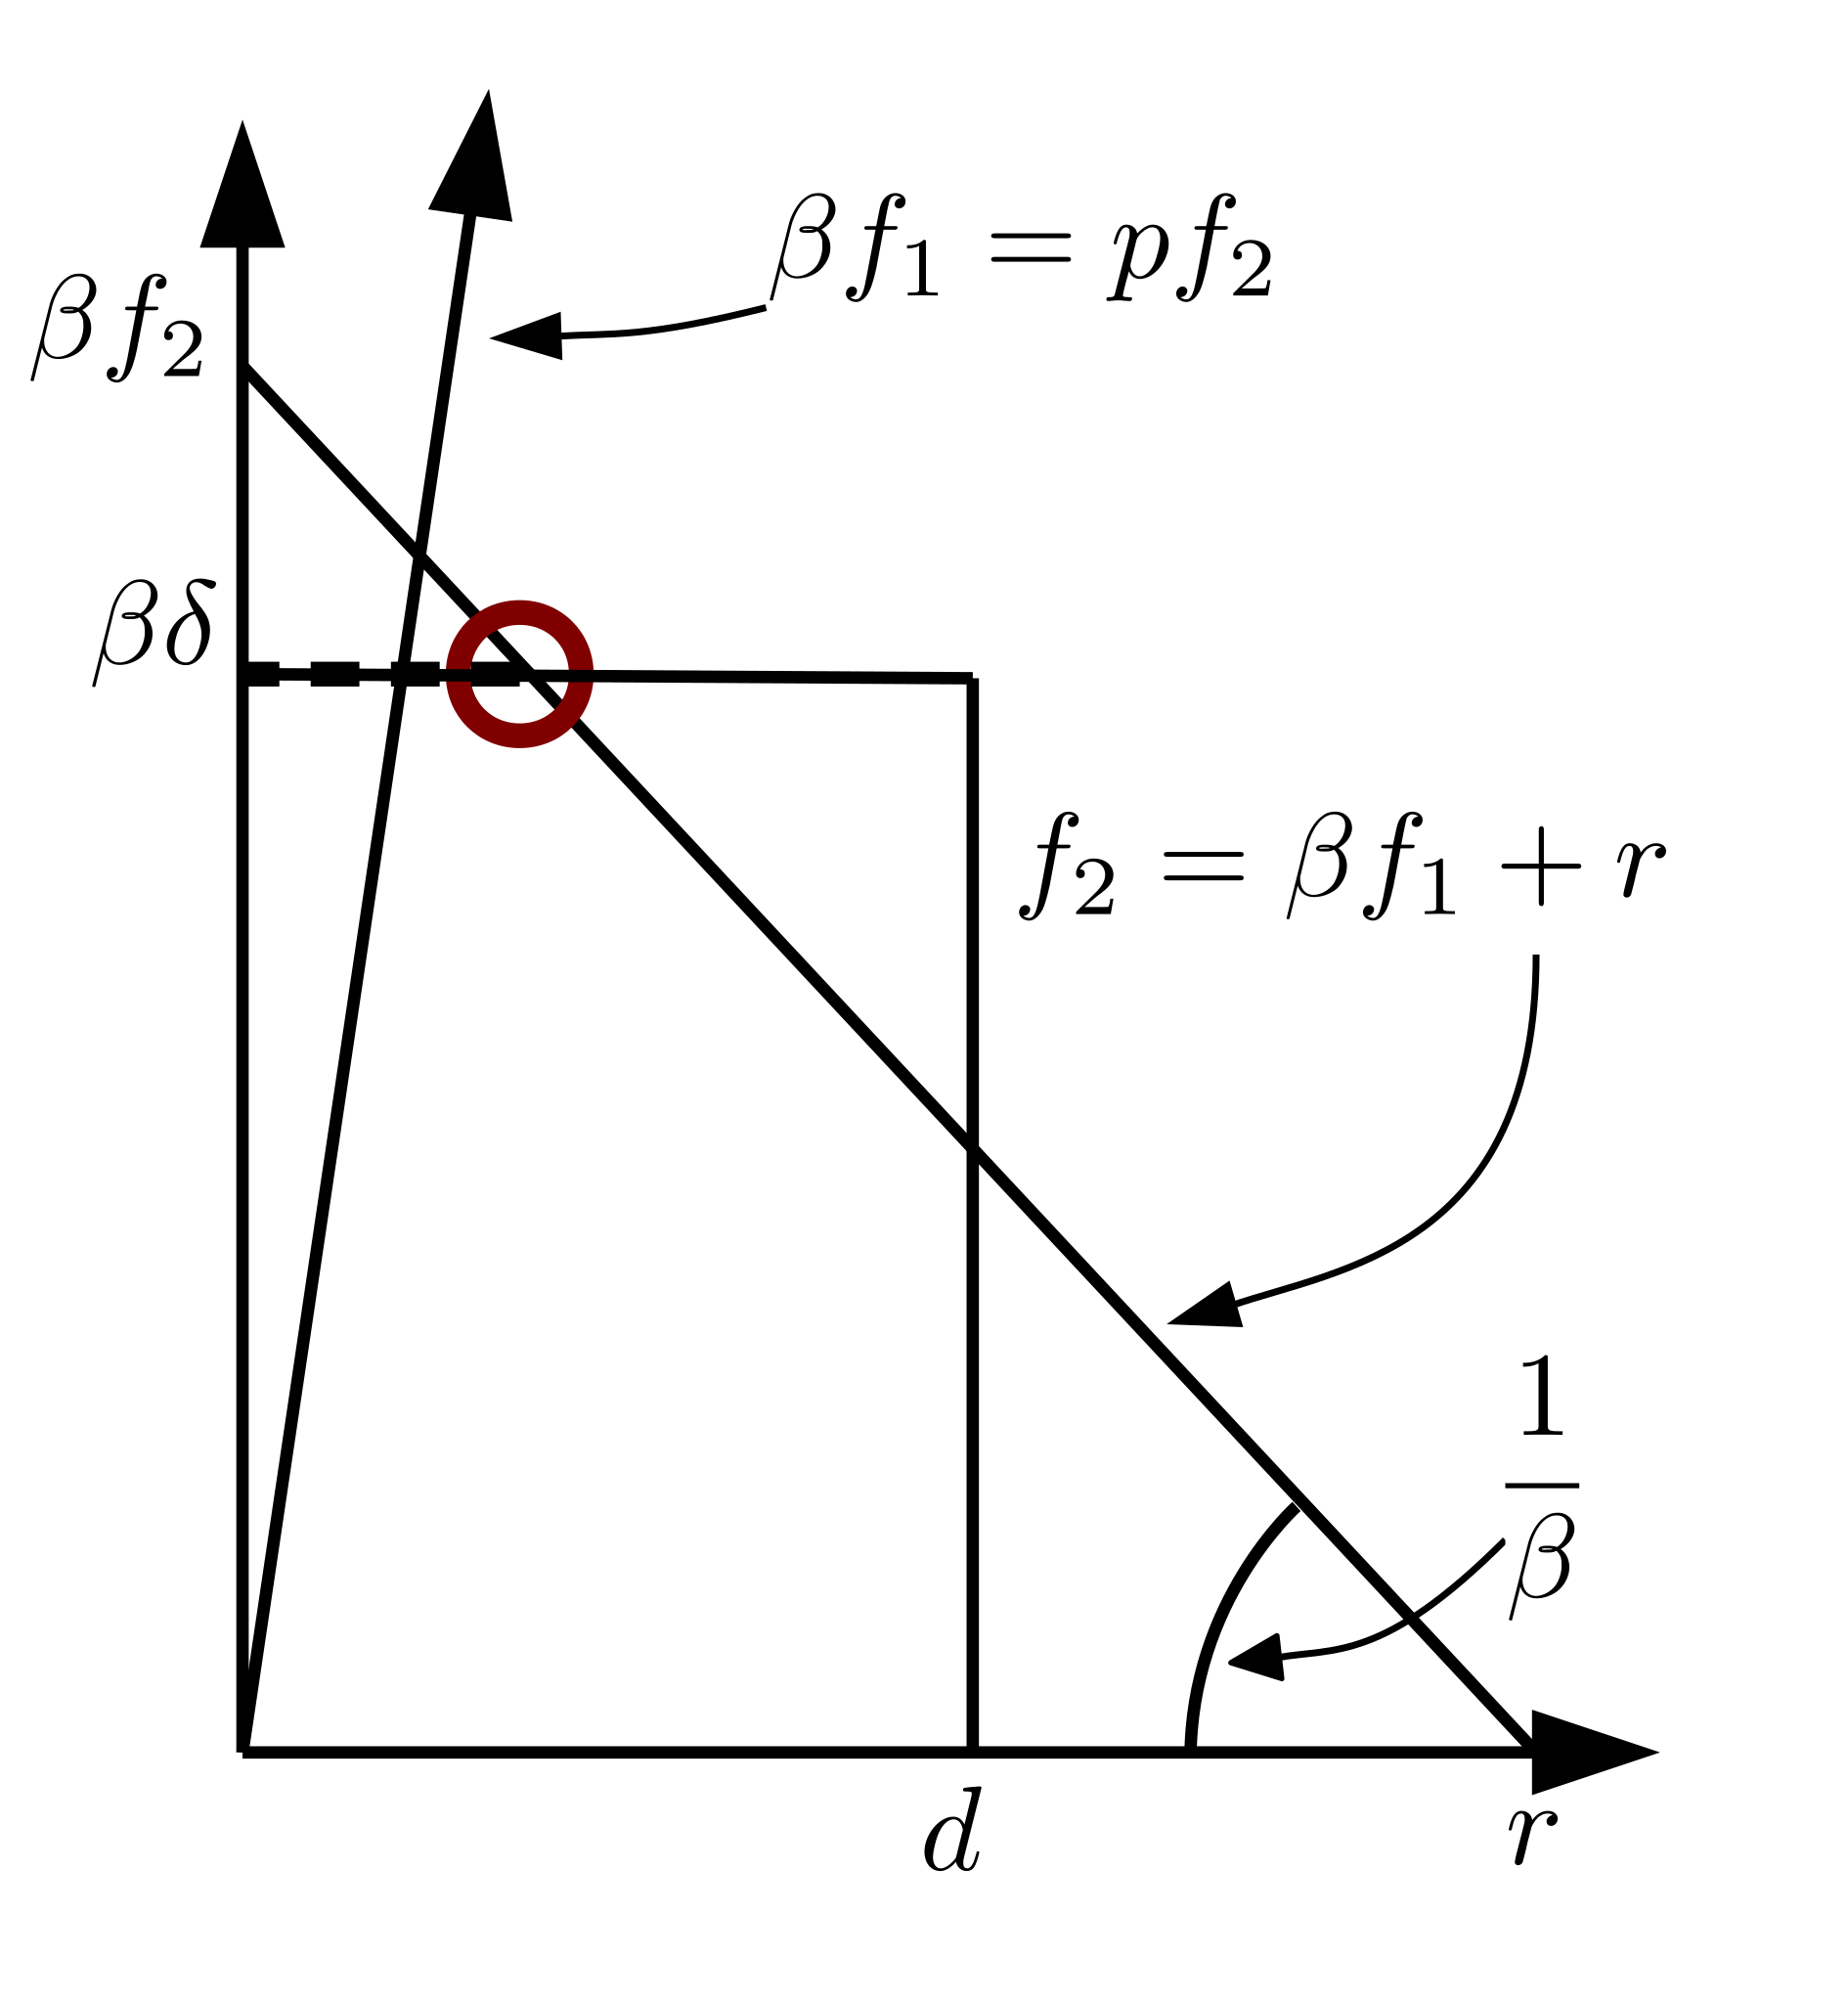
\includegraphics[width=0.25\columnwidth]{previous-articles/adjoint/figures/flux-sln-1}
}\hfill%
\subfloat[Case 2: Priority violated due to limited on ramp demand entering downstream
mainline.]{\includegraphics[width=0.25\columnwidth]{previous-articles/adjoint/figures/flux-sln-2-thesis}
}\hfill%
\subfloat[Case 3: Priority rule satisfied due to sufficient demand from both
mainline and on ramp.]{\includegraphics[width=0.25\columnwidth]{previous-articles/adjoint/figures/flux-sln-3-thesis}
}
\caption[Godunov junction flux solution for freeway model.]{Godunov junction flux solution for freeway model. The rectangular region represents the feasible flux
values for $I_1$ ($\beta \delta$) and $R_1$ ($d$) as determined by the upstream demand, while
the line with slope $\frac{1}{\beta}$
represents feasible flux values as determined by mass balance. The
$\beta f_1$
term accounts for only the flux out of $I_1$
that stays on the mainline. The flux solution, represented by the
red circle, is the point on the feasible region that minimizes the
distance from the priority line $f_1 = p r$.}
\label{fig:Godunov-junction-flux}
\end{figure}

To compute the flux leaving $I_1$, we refer to Figure~\ref{fig:Godunov-junction-flux}. The balance between the fluxes $\beta f_1$ (resp. $r$) entering $I_2$  from $I_1$ (resp. $R_1$) must minimize the deviation from the equation $\beta f_1 = p r$. Since flow must be conserved across the junction, we also have the constraint that the $\left(\beta f_1, r\right)$ flows must sum to $f_2$, and thus the resultant flow pair $\left(f_1, r\right)$ must lie on the line $f_2 = \beta f_1 + r$, depicted in Figure~\ref{fig:Godunov-junction-flux}. This results in three distinct cases for the $f_1$ solution.

\begin{itemize}
	\item In Case 1, strict satisfaction of the priority line would lead to an $f_1$ value greater than $\delta$ when at the intersection with the supply line $f_2 = \beta f_1 + r$. Since $\delta$ is the maximum allowable flux from $I_1$, we can feasibly exactly satisfy the priority. Thus to minimize the deviation from the priority line, we select $f_1 = \delta$.
	\item In Case 2, the priority dictates a flux from $R_1$ in excess of $d$. To minimize deviation from priority, we select $r = d$, and $\beta f_1 = f_2 - r$.
	\item In Case 3, strict satisfaction of the priority line gives a feasible $f_1$ and $r$ solution, and thus we have $f_1 = \frac{f_2}{\beta \left(1 + p^{-1}\right)}$.
\end{itemize}


Once we have determined $f_1$ and $f_2$, then flux balance across the junction dictates that $r = f_2 - \beta f_1$.

To satisfy the Riemann solver condition that only waves that travel outward from the junction may be created, we devise a mapping from the resultant mainline fluxes $\left(f_1, f_2\right)$ to the Riemann solver densities $\left(\hat{\rho}_1^+, \hat{\rho}_2^-\right)$. The following conditions uniquely determine $\left(\hat{\rho}_1^+, \hat{\rho}_2^-\right)$:

\begin{align}
\hat{\rho}_1^+ \in
\begin{cases}
\left\{\rho_1^+\right\}\cup ]\tau(\rho_1^+),\rho^{\max}] & \text{if } 0 \le \rho_1^+ \le \rho^\text{cr}, \\
\left[\rho^{\text{cr}}, \rho^{\max}\right] & \text{if }  \rho^\text{cr} \le  \rho_1^+ \le \rho^{\max};
\end{cases} &\quad  & f\left(\hat{\rho}_1^+\right) = f_1 \\
\hat{\rho}_2^- \in
\begin{cases}
\left[0,\rho^{\text{cr}}\right] & \text{if } 0 \le \rho_2^- \le \rho^\text{cr}, \\
 \left\{\rho_2^-\right\}\cup [0,\tau(\rho_2^-)]
 & \text{if }  \rho^\text{cr} \le  \rho_2^- \le \rho^{\max};
\end{cases} &\quad  & f\left(\hat{\rho}_2^-\right) = f_2,
\end{align}

where $\tau$ satisfies the following:

\begin{enumerate}
	\item $f(\tau(\rho)) = f(\rho)$
	\item $\tau(\rho) \neq \rho$
\end{enumerate}

\subsection{Discrete Freeway Model}

The previous section derives a continuous traffic model based on the principle of mass conservation and matching the empirical flux-density relationship. Furthermore, the model possesses strong boundary conditions, allowing for the total flux through the network to be independent of any varying control parameters.

In order to develop computationally efficient optimization and control techniques, we work in the discrete time and space domain. As detailed in Section~\ref{sec:godunov-discretization}, we use the Godunov discretization technique.

We now consider a freeway network with multiple junctions, as opposed to the presentation of the continuous model, which only considered a single junction.

Consider a freeway section with links $\links=\intrange 1{2\nlinks}$
with a linear sequence of mainline links $=\intrange{2,4}{2\nlinks}$
and connecting on ramp links $=\intrange{1,3}{2\nlinks-1}$. At discrete
time $t=\tind\Delta t,0\le\tind\le\ntime-1$, mainline link $2\link\in\links,i\in\intrange 1{\nlinks}$
has a downstream junction $\jdown{2\link}=\jup{2\left(\link+1\right)}$
and an upstream junction $\jup{2\link}=\jdown{2\left(\link-1\right)}$,
while on ramp $2\link-1\in\links,i\in\intrange 1{\nlinks}$ has a downstream
junction $\jdown{2\link-1}=\jup{2\link}=\jdown{2\left(\link-1\right)}$
and an upstream junction $\jup{2\link-1}$.

The off-ramp directly downstream of link $2\link,i\in\intrange 1{\nlinks}$
has, at time-step $\tind$, a split ratio $\splitratio_{2\link}^{\tind}$
Each link $\link\in\links$ has a discretized state value $\densitydiscrete{\link}{\tind}\in\mathbb{R}$
at each time-step $\tind\in\intrange 0{\ntime-1}$, that represents
the density of vehicles on the link. These values are depicted in
Fig~\ref{fig:Freeway-network-junction}. Junctions that have no
on ramps can be effectively represented by adding an on ramp with no
demand while junctions with no off-ramps can be represented by setting
the split ratio to 1.
\begin{figure}
\centering
\includegraphics[width=1\columnwidth]{previous-articles/adjoint/figs-gen/rm-junction-2}
\caption[Freeway network model depicting the discrete model notation on a single freeway/onramp junction.]{Freeway network model. For a junction $\jdown{2\link-1}=\jdown{2\left(\link-1\right)}=\jup{2\link}$
at time-step $\tind\in\intrange 0{\ntime-1}$, the upstream mainline
density are represented by $\densitydiscrete{2\left(\link-1\right)}{\tind}$,
the downstream mainline density by $\densitydiscrete{2\link}{\tind}$,
the on ramp density by $\densitydiscrete{2\link-1}{\tind}$, and the
off-ramp split ratio by $\splitratio_{2\left(\link-1\right)}^{\tind}$.}
\label{fig:Freeway-network-junction}
\end{figure}

As control input which is used extensively in applications in proceeding sections, an on ramp $2\link-1\in\links,\link\in\intrange 1{\nlinks}$
at time-step $k\in\intrange 0{\ntime-1}$ has a metering rate $\ramp_{2\link-1}^{\tind}\in\left[0,1\right]$
which limits the flux of vehicles leaving the on ramp. Intuitively,
the metering rate acts as a fractional decrease in the flow leaving
the on ramp and entering the mainline freeway. The domain of the metering
control is to force the control to neither impose negative flows nor
send more vehicles than present in a queue. Its mathematical model
is expressed in~\eqref{eq:ramp-eqn}.

For notational simplicity we define the set of densities of links
incident to $\jup{2\link}=\jdown{2\left(\link-1\right)}$ at time-step
$\tind$ as $\juncstate{\jup{2\link}}{\tind}=\left\{ \discrete{2\left(\link-1\right)}{\tind},\discrete{2i-1}{\tind},\discrete{2\link}{\tind}\right\} $. For $k\in\intrange 1{\ntime-1}$,
the mainline density $\discrete{2\link}{\tind}$ using the Godunov
scheme from~\eqref{eq:godscheme} is given by:

\begin{eqnarray}
\syseq_{2\link}^{\tind}(\state,\control)= & \discrete{2\link}{\tind}-\discrete{2\link}{\tind-1} & +\dfrac{\Delta t}{\length_{2\link}}\left(\god_{\jdown{2\link}}\left(\juncstate{\jdown{2\link}}{\tind-1},\ramp_{2\link+1}^{\tind-1}\right)\right)_{2\link}\label{eq:rho-update}\\
&  & -\dfrac{\Delta t}{\length_{2\link}}\left(\god_{\jup{2\link}}\left(\juncstate{\jup{2\link}}{\tind-1},\ramp_{2\link-1}^{\tind-1}\right)\right)_{2\link}\nonumber \\
= & \discrete{2\link}{\tind}-\discrete{2\link}{\tind-1} & +\frac{\Delta t}{\length_{2\link}}\left(\fout{2\link}{\tind-1}-\fin{2\link}{\tind-1}\right)=0
\end{eqnarray}
where we have introduced some substitutions to reduce the notational
burden of this section: $\fout{\link}{\tind}$ is the Godunov flux
at time-step $\tind$ exiting a link $\link$ at the downstream boundary
of the link, and $\fin{\link}{\tind}$ is the Godunov flux entering
the link at the upstream boundary.

We also make the assumption that on ramps have infinite capacity and
a free-flow velocity $\ffspeed_{2\link-1}=\frac{\length_{2\link-1}}{\Delta t}$
to prevent the ramp congestion from blocking demand from ever entering
the network. Since the on ramp has no physical length, the length
is chosen arbitrarily and the ``virtual'' velocity chosen above
is chosen to replicate the dynamics in~\cite{delle2014pde}. We can
then simplify the on ramp update equation to be:

\begin{eqnarray}
\syseq_{2\link-1}^{\tind}(\state,\control) & = & \discrete{2\link-1}{\tind}-\discrete{2\link-1}{\tind-1}-\frac{\Delta t}{\length_{2\link-1}}\left(\left(\god_{\jup{2\link}}\left(\juncstate{\jup{2\link}}{\tind-1},\ramp_{2\link-1}^{\tind-1}\right)\right)_{2\link-1}-\boundaryDemand{2\link-1}{\tind-1}\right)\label{eq:on ramp-update}\\
& = & \discrete{2\link-1}{\tind}-\discrete{2\link-1}{\tind-1}-\frac{\Delta t}{\length_{2\link-1}}\left(\fout{2\link-1}{\tind-1}-\boundaryDemand{2\link-1}{\tind-1}\right)=0
\end{eqnarray}
where $\boundaryDemand{2\link-1}{\tind-1}$ is the on ramp \emph{flux
}demand, and the same notational simplification has been used for
the downstream flux. This formulation results in ``strong'' boundary
conditions at the on ramps which guarantees all demand enters the network.

The on ramp model in~\eqref{eq:on ramp-update} differs from~\cite{delle2014pde}
in that we model the on ramp as a discretized PDE with an infinite
critical density, while~\cite{delle2014pde} models the on ramp
as an ODE ``buffer''. While both models implement strong boundary
conditions, the discretized PDE model makes the freeway network more
aligned with the PDE network framework presented in this section.

\paragraph{Discrete Model Equations}



The following systems of equations give the flux
solution of the Riemann solver at time-step $k\in\intrange 1{\ntime-1}$
and junction $\jup{2\link}$ for $\link\in\intrange 1{\nlinks}$:

\begin{eqnarray}
\demand_{2\left(\link-1\right)}^{\tind} & = & \min\left(\ffspeed_{2\left(i-1\right)}\densitydiscrete{2\left(\link-1\right)}{\tind},F_{2\left(\link-1\right)}^{\max}\right)\label{eq:first-ramp}\\
\supply_{2\link}^{\tind} & = & \min\left(\congspeed_{2i}\left(\density_{2i}^{\max}-\densitydiscrete{2\link}{\tind}\right),F_{2i}^{\max}\right)\label{eq:supply}\\
\rampDemand_{2\link-1}^{\tind} & = & \ramp_{2\link-1}^{\tind}\min\left(\frac{\length_{2\link-1}}{\Delta t}\densitydiscrete{2\link-1}{\tind},F_{2i-1}^{\max}\right)\label{eq:ramp-eqn}\\
\fin{2\link}{\tind} & = & \min\left(\splitratio_{2\left(\link-1\right)}^{\tind}\demand_{2\left(\link-1\right)}^{\tind}+\rampDemand_{2\link-1}^{\tind},\supply_{2\link}^{\tind}\right)\label{eq:fin}\\
\fout{2\left(\link-1\right)}{\tind} & = & \begin{cases}
\demand_{2\left(\link-1\right)}^{\tind} & \frac{p_{2(\link-1)}\fin{2\link}{\tind}}{\splitratio_{2\left(\link-1\right)}^{\tind}\left(1+p_{2(\link-1)}\right)}\ge\demand_{2\left(\link-1\right)}^{\tind}\hfill\text{[Case 1]}\\
\frac{\fin{2\link}{\tind}-\rampDemand_{2\link-1}^{\tind}}{\splitratio_{2\left(\link-1\right)}^{\tind}} & \frac{\fin{2\link}{\tind}}{1+p_{2(\link-1)}}\ge\rampDemand_{2\link-1}^{\tind}\hfill\text{[Case 2}]\\
\frac{p_{2(\link-1)}\fin{2\link}{\tind}}{\left(1+p_{2(\link-1)}\right)\splitratio_{2\left(\link-1\right)}^{\tind}} & \text{otherwise}\hfill[\text{Case 3]}
\end{cases}\label{eq:merge}\\
\fout{2\link-1}{\tind} & = & \fin{2\link}{\tind}-\splitratio_{2\left(\link-1\right)}^{\tind}\fout{2\left(\link-1\right)}{\tind}\label{eq:last-ramp}
\end{eqnarray}
where, for notational simplicity, at the edges of of the range for
$\link$, any undefined state values (e.g. $\densitydiscrete 0{\tind}$)
are assumed to be zero by convention. 

Note that the equations can be solved sequentially via forward substitution. Also, we do not include
the flux result for off-ramps explicitly here since its value has no
bearing on further calculations, and we will henceforth ignore its
calculation. To demonstrate that indeed the flux solution satisfies
the flux conservation property, the off-ramp flux is trivially determined
to be $\splitratio_{2\left(\link-1\right)}^{\tind}\fout{2\left(\link-1\right)}{\tind}$.

\chapter{Centralized and Decentralized Optimal Freeway Control via the Discrete Adjoint Method}

\section{Discrete Adjoint Derivation for Networked Conservation Laws}

\subsection{Discrete Adjoint Overview}

\subsection{Application to Networked Conservation Laws}

\subsection{Complexity Analysis of Discrete Adjoint for Sparse Networks}

\section{Adjoint-based Model Predictive Control for Coordinated, Predictive Ramp Metering}

\subsection{Partial Derivative Calculations for Ramp Metering}

\subsection{Model Predictive Control Overview}

\subsection{Numerical Results}
\label{sec:numerical-results-adjoint}
\section{Decentralized Control of Flow Networks}
\label{sec:admm-intro}

Finite-horizon optimal control is a popular method for computing predictive control strategies for dynamical systems~\cite{Reilly2013AdjointBased,Bayen2006AdjointBased,Raffard2008AdjointBased}, its applicabilibity growing with the increase of computational power and pervasiveness of physical sensing. In general, a finite-horizon optimal control problem will take the following form:

\begin{align}
	\label{eq:fhop}
	\min_{x\in X} & \quad f\left(s, x\right) \\
	\text{subject to:} & \quad s = g\left(x\right)
\end{align}

where $x$ represents the vector of control variables belonging to the set of feasible controls $X$ (which we may assume to be $\Re^n$ for simplicity), $s$ represents the vector of ``state'' variables, constrained to be a deterministic function $g\left(x\right)$ of the control, and $f$ is some objective function of the control and state we wish to minimize.

\paragraph*{Related Work in Distributed Optimization}
Much attention has recently been given to distributed methods for finite-horizon optimal control problems, where $g$ is assumed to be linear and $f$ is assumed to be quadratic or convex. Distributed optimization has been found useful for at least two reasons. Firstly, the parallelizability of the individual sub-problems allows for faster computation time and better overall convergence properties~\cite{Donoghue2013Splitting,Frejo2011Feasible,Pu2014Fast,Giselsson2013Accelerated}. Secondly, physical systems often have their controls physically distributed in space, creating a need for distributed control algorithms which limit the amount of shared information and communication between subsystems~\cite{Venkat2008Distributed,mota2012distributed,camponogara2009distributed}.

Different assumptions on the structure, smoothness, and convexity of $f$, $X$ and $g$ leads to different convergence bounds and communication bounds in distributed optimization. A method for decoupling the quadratic terms from the nonquadratic terms in optimal control, presented in~\cite{Donoghue2013Splitting} leads to efficient caching techniques shown to be effective in FPGA applications. A distributed gradient descent-based approach is given in~\cite{camponogara2009distributed}, which has $O\left(\frac{1}{\sqrt{k}}\right)$ convergence to the global optimum in the general case, where $k$ is the number of iterations of the algorithm.  A common dual-decomposition technique employed for distributed optimal control is the \emph{alternating directions method of multipliers}~\cite{Boyd2010Distributed,Donoghue2013Splitting,gabay1976dual} (ADMM), which has been shown to have $O\left(\frac{1}{k}\right)$ convergence under certain assumptions of the smoothness and decomposability of the objectives~\cite{Wei2013On}. Additionally, an accelerated version of ADMM, based on Nesterov's algorithm~\cite{Nesterov1983Method} can give $O\left(\frac{1}{k^2}\right)$ convergence when the decomposed objectives are smooth~\cite{Pu2014Fast}.

When the coupling between systems takes on some sparse form, then one can devise algorithms with limited communication, which can be beneficial from a latency and  architectural standpoint. Optimal control problems where subsystems have disjoint state variables but coupled control variables have been shown to be amenable to decomposition techniques for distributed optimization~\cite{Giselsson2013Accelerated,camponogara2009distributed}, where~\cite{mota2012distributed} shows how ADMM decomposition leads to less communication without a decrease in solution accuracy.

In~\cite{Giselsson2013Accelerated,mota2012distributed,camponogara2009distributed}, the subsystems with disjoint state are modeled as agents tasked with optimizing over their own subsystem, where agents which share some control variables are connected by some edge in a communication graph. Thus, the more sparse the coupling of systems, the lesser the communication requirements. Such a model is referred to as \emph{multi-agent optimization}~\cite{Wei2013On}. In systems with coupling due to physical proximity, this consequence has the added benefit of requiring only physically local communication, and removes the need for any centralized controller or hub for communication. In~\cite{Wei2013On}, an asynchronous form of ADMM (subsequenetly referred to as A-ADMM) is presented for multi-agent optimization, which permits agents to update themselves in arbitrary order, with communication only required between neighboring agents. The method in~\cite{Wei2013On} does not present an accelerated version and is shown to have $O\left(\frac{1}{k}\right)$ convergence.

\paragraph*{Subsystems with Coupled State}
One recurring assumption in the distributed optimization literature above is that subsystems have disjoint state variables. For network flow problems, where subsystems correspond to partitions of a network into subnetworks, such an assumption does not hold. To see this, one can imagine a traffic light timing plan causing a traffic jam which spreads across the entire freeway network~\cite{Reilly2013AdjointBased,Muralidharan2012Optimal} or a bottleneck of planes in an airspace affecting flight times throughout the air network~\cite{Bayen2006AdjointBased}. As a result, it is not possible to decompose the subsystems by only sharing control parameters without coupling each subsystem to all control variables and modeling the evolution of the entire network within each subsystem.

Yet, freeway traffic and air traffic subsystems have a very sparse coupling in their state variables. For instance, discrete traffic models~\cite{Monache2014PdeOde,daganzo1995cell} often assume that the speed of traffic on a particular section of road is only a function of the speed of traffic on neighboring links. Thus, each subnetwork subsystem would only share a small number of control variables and state variables with other subsystems, precisely those which physically share a border with the subsystem.

To exploit the sparsity of such systems, we develop a multi-agent optimization algorithm based on A-ADMM~\cite{Wei2013On} which permits each agent (subsystem) to share both control and state variables with neighboring agents, while still converging to the globally optimal control, given the standard assumption of convex objectives and linear constraints. At a high level, the algorithm ``relaxes'' the state variables \emph{external} to an agent while constraining \emph{internal} state variables to adhere to the subsystem's dynamics. Since A-ADMM eventually brings all shared variables between agents into \emph{consensus} (i.e. the difference between shared variables converges to zero), the relaxed external state variables will converge to satisfying the original constraints.

The rest of the section is structured as follows.
% Section~\ref{sec:admm-overview} gives an overview of ADMM and its application to consensus-type problems.
Section~\ref{sec:problem_statement} presents the general problem of posing a multi-agent optimal control problem, with the additional assumption that an agent may share both state and control variables with other agents. The problem is then posed in a form amenable to using the A-ADMM algorithm in Section~\ref{sec:algorithm}. A systematic approach to modeling an optimal control problem over a dynamical network as a multi-agent distributed optimization over subnetworks is given in Section~\ref{sec:distributed_optimization_of_coupled_dynamical_systems}, as well as a discussion on the suitability of the method for scaling model predictive control on dynamical networks. In Section~\ref{sec:minimizing_sub_objectives_using_the_adjoint_method}, we give an adjoint-based approach to solving the agent's subnetwork optimal control problem, suitable for applications with complex, non-convex dynamics. We then present the application of distributed, predictive ramp-metering control on freeway networks in Section~\ref{sec:ramp-metering-admm} followed by numerical results in Section~\ref{sec:numerical_results-admm} with comparisons to existing distributed approaches.
% We conclude with some final remarks in Section~\ref{sec:conclusion}.

\paragraph*{\textbf{Notation}}

For a vector $x$, let $x\left[i\right]$ be the $i$'th element of $x$, and similarly let $y\left[i,j\right]$ be the element of the two-dimensional vector in the $i$'th row and $j$'th column. If we have a vector $x$ with $card\left(x\right)=N$ and let $w$ be a subset of $ \{1,\ldots,N\}$, then let $x_w$ denote the vector selecting only those elements $x\left[i\right]$ where $i\in w$. If a vector $d$ is the concatenation $d = \left(a,b,c\right)$, then let $\left[d\right]_a$ be the sub-vector of $d$ corresponding to the original element $a$.

% \subsection{Distributed Optimization and ADMM}
% \label{sec:admm-overview}

% \todo{overview of admm and distributed optimization.}

\subsection{Optimization over Systems with Shared State}
\label{sec:problem_statement}

We wish to solve an optimization problem with a ``free'' global variable $x \in \Re^n$ and a ``dependent'' variable $s \in \Re^m$ which is a deterministic function of $x$.
We assume there is a partition of $s$ into $D$ disjoint subsets,
\[
s=\left(s_{u\left(1\right)},\ldots,s_{u\left(D\right)}\right),
\] where $u\left(i\right)$ are subsets of $ \{1,\ldots,m\} $.
The objective function is assumed to be the sum of $D$ sub-objectives, where sub-objective $f_i, i\in \{1,\ldots,D\} $ is a convex function of only variable $s_{u\left(i\right)}$~\footnote{We omit the dependency of the objective on the control variable in this presentation for simplicity. It is still easy in this form to add control variables into the objective by duplicating a control variable into the state.}.
Furthermore, $s_{u\left(i\right)}$ is assumed to be a function of some subset of $x$ and $s$.
Explicitly, for each $i\in {1,\ldots, D} $, there is well-defined, linear function $g_i$ and subsets $v\left(i\right)$ and $w\left(i\right)$ ($w\left(i\right) \cap u\left(i\right) = \emptyset$) where 
\[
s_{u\left(i\right)} = g_i\left(\left(x_{v\left(i\right)}, s_{w\left(i\right)}\right)\right).
\]
The tuple $\left(x_{v\left(i\right)}, s_{w\left(i\right)}\right)$ is the concatenation vector of $x_{v\left(i\right)}$ and $s_{w\left(i\right)}$.
We omit the double parenthesis in the rest, for simplicity. One can view $u\left(i\right), v\left(i\right), w\left(i\right), $ as the \emph{internal} state, the control, and the \emph{external} state, respectively, of group $i$. 
We can now express the optimization problem we wish to solve as:

\begin{align}
	\label{eq:problem-statement}
	\min_{x,s} & \quad \sum_{i = 1}^D f_i\left(s_{u\left(i\right)}\right) \\
	\text{subject to:} & \quad s_{u\left(i\right)} = g_i\left(x_{v\left(i\right)}, s_{w\left(i\right)}\right) \quad \forall i
\end{align}

Figure~\ref{sub:dep-graph-diagram} shows an example of how different sub-objectives may be coupled and Table~\ref{tab:dep-graph-subsets} summarizes how one constructs the $u\left(i\right), v\left(i\right), w\left(i\right)$ subsets from the state and control coupling.

\begin{figure}[t]
\centering
	\subfloat[Free and dependent variable coupling diagram.]{%
	\label{sub:dep-graph-diagram}%
	\includegraphics[width=.45\columnwidth]{previous-articles/admm/figures/dep-graph}
	}\\
	\subfloat[Summary of resultant state, control, and external state subsets.]{%
    \begin{tabular}{|l|c|c|c|}
    \hline
    Group $i$ & $u\left(i\right)$ & $v\left(i\right)$ & $w\left(i\right)$\\ \hline
    $i=1$ & \{1,2\}       & \{1\}        & \{\}        \\ \hline
    $i=2$ & \{3\}        & \{1,2\}       & \{4,5\}       \\ \hline
    $i=3$ & \{4,5\}        & \{3\}       & \{3\}       \\ \hline
    \end{tabular}\label{tab:dep-graph-subsets}}\hfill%
    \subfloat[Summary of shared control and state between groups]{
    \begin{tabular}{|l|c|c|c|}
    \hline
    Edge $\left(i,j\right)$ & $v\left(i\right) \cap v\left(j\right)$ & $u\left(i\right) \cap w\left(j\right)$ & w$\left(i\right) \cap u\left(j\right)$  \\ \hline
    $i,j=1,2$ & \{1\}       & \{\}        & \{\}        \\ \hline
    $i,j=2,3$ & \{\}        & \{3\}       & \{4,5\}       \\ \hline
    $i,j=1,3$ & \{\}        & \{\}       & \{\}       \\ \hline
    \end{tabular}
\label{tab:dep-graph-edges}
}
    \caption{Example of optimization problem partitioned into $D=3$ disjoint state variable groups with shared control and external state variables. Figure~\ref{sub:dep-graph-diagram} shows the partitioned problem, where an arrow depicts a dependency of a partition group on an external state variable or control variable. The arrows allow us to compute the $u\left(i\right), v\left(i\right), w\left(i\right)$ subsets for each group $i$, which is summarized in Table~\ref{tab:dep-graph-subsets}. The dependency graph $(V,E)$ is computed using the subsets in Table~\ref{tab:dep-graph-subsets}, which is summarized in Table~\ref{tab:dep-graph-edges} and reveals that edges exist for groups $\left(1,2\right)$ and $\left(2,3\right)$, but not for $\left(1,3\right)$.}%
    \label{fig:dep-graph}
  \end{figure}


\paragraph*{Dependency Graph}

There are no assumptions on the subsets $v\left(i\right)$ and $w\left(i\right)$, which implies that the value of each sub-objective $f_i$ is coupled to not just the sub-vector $s_{u\left(i\right)}$, but also the global variable $x$, and other sub-vectors $s_{u\left(j\right)}$. We can express this coupling as a dependency graph $\left(V,E\right)$, where vertices $V$ are each sub-problem $i\in \{1,\ldots, D\} $ and an edge $\left(i,j\right)\in E$ exists whenever

\begin{enumerate}
	\item  $w\left(i\right) \cap u\left(j\right) \neq \emptyset$ ($g_i$ is a function of some variable in $s_{u\left(j\right)}$), \textbf{or}
	\item $v\left(i\right) \cap v\left(j\right) \neq \emptyset$ (there is some $x\left[k\right]$ which both $g_i$ and $g_j$ depend upon).
\end{enumerate}
 
Let the neighboring edges of node $i\in V$ be denoted by $E\left(i\right)$. A dependency graph construction for the example in Figure~\ref{sub:dep-graph-diagram} is summarized in Table~\ref{tab:dep-graph-edges}.

In Section~\ref{sec:algorithm}, we devise a distributed algorithm solve Problem~\eqref{eq:problem-statement} with the following requirements:

\begin{enumerate}
	\item Each processing node corresponds to a sub-objective node in the dependency graph.
	\item Each node can be updated in parallel.
	\item Each node $i$ only exchanges information with its neighbors $E\left(i\right)$ in the dependency graph $\left(V,E\right)$.
	\item The algorithm is asynchronous and decentralized, i.e. no central process is required and nodes can be updated arbitrarily.
\end{enumerate}

% \subsection{Asynchronous ADMM and Subnetwork Splitting}
% \label{sec:algorithm}

% section problem_statement (end)

\subsection{Asynchronous-ADMM Algorithm} % (fold)
\label{sec:algorithm}

We now reformulate Problem~\eqref{eq:problem-statement} to permit a distributed solution method via A-ADMM.  For each node $i\in V$, we replicate the ``shared variables'' $x_{v\left(i\right)}$ and $s_{w\left(i\right)}$ as $\bar{x}_i$ and $\bar{s}_i$ respectively, and reformulate Problem~\eqref{eq:problem-statement} as:

\begin{align}
	\label{eq:replicate-problem-statement}
	\min_{x} & \quad \sum_{i = 1}^D f_i\left(s_{u\left(i\right)}\right) \\
	\text{subject to:} & \quad s_{u\left(i\right)} = g_i\left(\bar{x}_i, \bar{s}_i\right) \quad \forall i  \label{eqn:state-constraint-decoupled} \\
	 & \quad \bar{s}_i = s_{w\left(i\right)} \quad \forall i \label{eqn:state-consensus} \\
	 & \quad \bar{x}_i = x_{v\left(i\right)} \quad \forall i \label{eqn:control-consensus} 
\end{align}

The variable replication allows Constraint~\eqref{eqn:state-constraint-decoupled} in Problem~\eqref{eq:replicate-problem-statement} to be decoupled across nodes. To decouple Constraints~\eqref{eqn:state-consensus} and~\eqref{eqn:control-consensus}, we follow a modified process from~\cite{Wei2013On}.

First, we replicate each subset $s_{u\left(i\right)}$ with a vector $s_i$ local to node $i \in V$, and then concatenate all local variables into a single variable $y_i = \left(s_i, \bar{x}_i, \bar{s}_i\right)$, such that $y_i$ is restricted to the space:
\[
Y_i = \{\left(s_i,\bar{x}_i, \bar{s}_i\right) : s_i = g_i\left(\bar{x}_i, \bar{s}_i\right)\}.
\]
Finally, we can repose Constraints 2 and 3 in an \emph{edge-wise} fashion as follows. For each edge $e = \left(i,j\right) \in E$, let $y_{i,e}$ and $y_{j,e}$ be the sub-vectors of $y_i$ and $y_j$ that are coupled through $g_j$ and $g_i$, respectively. Then Problem~\eqref{eq:problem-statement} becomes:

\begin{align}
	\label{eq:edge-problem-statement}
	\min_{(y_i \in Y_i)_{i \in V}} & \sum_{i = 1}^D f_i\left(\left[y_i\right]_{s}\right) \\
	\text{subject to:} & \quad y_{i,e} = y_{j,e} \quad \forall e\in E
\end{align}

By moving the edge constraints into the objective through a standard Lagrange multiplier approach, and adding a regularization term which is equal to zero for feasible solutions~\cite{Boyd2010Distributed}, we can construct the augmented Lagrangian $\mathcal{L}$ formulation (with tunable augmenting coefficient $\augterm$), and express the optimization problem as:

\begin{align}
	\label{eq:lagrangian}
	\min_{y = (y_i)_{i \in V}} \max_{\lambda = \left(\lambda_e\right)_{e \in E}} & \mathcal{L} \left(y,\lambda\right) :=  \\
	& \sum_{i = 1}^D f_i\left(\left[y_i\right]_{s}\right) + \\
	& \sum_{e\in E} \lambda_e^T \left(y_{i,e} - y_{j,e}\right) + \augterm \|y_{i,e} - y_{j,e}\|_2^2, \nonumber
\end{align}
	
The above form permits us to apply the A-ADMM algorithm as proposed and analyzed in~\cite{Wei2013On}, and shown in Algorithm~\ref{alg:a-admm}. At a high-level, the algorithm iterates by first randomly selecting an edge $e = \left(i,j\right)$ from $E$. Then, nodes $i$ and $j$ update $y_i$ and $y_j$ respectively by minimizing the Lagrangian in Equation~\eqref{eq:lagrangian} in parallel, while holding all other variables $\{\lambda_e'\}_{e' \neq e}, \{y_k\}_{i\notin \{i,j\}}$ constant. The new $y_i$ and $y_j$ values are used to update the dual $\lambda_e$ variables by applying a dual-ascent method~\cite{Boyd2010Distributed}. Finally, the process is repeated \emph{ad-infinitum} by updating a new edge selected from $E$, until some convergence or termination criteria are reached.

Section~\ref{sec:minimizing_sub_objectives_using_the_adjoint_method} presents an efficient solution method, based on discrete adjoint computations, to solving the subproblem on Line 4 of Algorithm~\ref{alg:a-admm}.

\begin{remark} The equation in Line~\ref{lst:local-state-update} differs slightly from the augmented Lagrangian in Equation~\eqref{eq:lagrangian} and is the result of a number of algebraic manipulations, which are explicitly derived in~\cite{Boyd2010Distributed,Wei2013On}.
\end{remark}
\begin{remark}
We introduce the asymmetric coefficient $\Lambda_{q,e}$ to account for the fact that the terms for edge $e\in E\left(q\right)$ in Line~\ref{lst:local-state-update} depend upon whether the updating problem $q$ was the first or second term ($i$ or $j$) in the edge pair.
\end{remark}

\begin{algorithm}[t]  % enter the algorithm environment
\caption{Asynchronous Edge Based ADMM} % give the algorithm a caption
\label{alg:a-admm}       % and a label for \ref{} commands later in the document
\begin{algorithmic}[1]% enter the algorithmic environment
    \WHILE{Not Converged}
    \STATE Select edge $\left(i,j\right) \in E$
        \FOR{$q \in \left(i,j\right)$}
        \STATE $ y^{k+1}_q \gets \arg \min_{y \in Y_q} f_q\left(\left[y\right]_{s}\right) - \sum_{e \in E\left(q\right)}
        \Lambda_{q,e} \lambda^{k,T}_{e} \left(y_{q,e} - \bar{y}^{k}_{e} \right) +
        \frac{\augterm}{2} \|y_{q,e} - \bar{y}^{k}_{e}\|_2^2 $ \label{lst:local-state-update}
        \ENDFOR
        \STATE $\lambda^{k+1}_{e} \gets \lambda^{k+1}_{e} - \frac{\augterm}{2} \left(y^{k+1}_{i,e} - y^{k+1}_{j,e}\right)$
        \FOR{$q \notin \left(i,j\right)$}
        \STATE $a^{k+1} \gets a^{k}$
        \ENDFOR
    \ENDWHILE
    \STATE Note: $\tilde{y}^{k}_{e} = \frac{1}{2} \left(y^k_{i,e} + y^k_{j,e}\right)$
    \STATE Note: $\Lambda_{q,e} = \begin{cases} 1 & \quad q = i \\ -1 & \quad q = j \end{cases} \quad e = (i,j)$
\end{algorithmic}
\end{algorithm}

% section minimizing_sub_objectives_using_the_adjoint_method (end)

\subsection{Distributed Optimization on Coupled Dynamical Systems} % (fold)
\label{sec:distributed_optimization_of_coupled_dynamical_systems}

Physical transport systems, such as freeway traffic networks~\cite{Reilly2013AdjointBased,daganzo1995cell} or gas pipelines~\cite{Gugat2011Gas} are often naturally expressed as a network of individual dynamical systems which influence one another at contact points, or \emph{junction points}. Given the coupling in dynamics across the entire network, optimizating over partitioned sub-systems, with no communication between systems, will lead to \emph{greedy} solutions over the individual systems and sub-optimal global results~\cite{Ramon2013}. Thus, any distributed, globally optimal control scheme applied to such systems must account for the \emph{shared state} between the systems. We now show how this can be done using the multi-agent A-ADMM approach. Furthermore, we show how the algorithm naturally leads to a communication scheme which mirrors the physical structure of the underlying physical network.

Assume have some discrete-time, discrete-space dynamical system which possesses some network-like dynamical coupling in space. Specifically, consider a graph $\left(V^d, E^d\right)$ (not to be confused with the dependency graph $\left(V,D\right)$ in Section~\ref{sec:problem_statement}, where the $d$ superscript is added to denote the \emph{dynamical} network) where $E^d$ represent the discrete-space \emph{cells} and $V^d$ are the \emph{junction points} where cells connect to one another, i.e. each cell in $E^d$ has a corresponding upstream and downstream junction both in $V^d$.  Each discrete space ``cell'' $c \in \{1,\ldots,N_d\} $ has for each discrete time step $k \in \{1,\ldots,T_d\} $ both a control variable $x\left[c,k\right] \in \Re$ and a state variable $s\left[c,k\right] \in \Re$. The variable $s\left[c,k\right]$ is assumed to be a function of all state and control variables that satisfy two conditions:

\begin{itemize}
	\item the time-step is $k-1$, and
	\item the cell must share a junction with cell $c$.
\end{itemize}

Next, we wish to express a distributed optimization problem subject to the above dynamics in the form of Problem~\eqref{eq:problem-statement}. To do so, we assume a partition of $\left(V^d,E^d\right)$ into $D$ \emph{sub-networks}, which implies a partition of $E^d$ into $D$ subsets $\left(E^d_1,\ldots, E^d_D\right)$ and assume an objective $f$ which is splittable across the state variables internal to each sub-network. This leads to a state partitioning $s=\left(s_{u\left(1\right)}, \ldots, s_{u\left(D\right)}\right)$, where $ \left(c,k\right) \in u\left(i\right)$ iff $c \in E^d_i$.

Based on the two conditions for state dependencies above, we can deduce that the state of a sub-network depends on the control and state both internal to the sub-network and directly \emph{neighboring} the sub-network. Explicitly, for sub-network $i$, we can express the dependent control variables as $x_{v\left(i\right)}$ where $\left(c,k\right)\in v\left(i\right)$ iff $c \in E^d_i$ or $c$ neighbors a cell in $E^d_i$. Similarly, the shared state for sub-network $i$ is $s_{w\left(i\right)}$, where $\left(c,k\right)\in w\left(i\right)$ iff $c \notin E^d_i$ and $c$ neighbors a cell in $E^d_i$. Finally, we conclude that there exists some update equation $g_i$, specific to the particular dynamical system, where the constraint on $s_{u\left(i\right)}$ can be expressed familiarly as $s_{u\left(i\right)} = g_i\left(x_{v\left(i\right)}, s_{w\left(i\right)}\right)$.

\begin{figure}
	\subfloat[Complete network]{
	\includegraphics[width=.4\columnwidth]{previous-articles/admm/figures/net-1}
	\label{subfig:net-1}
	} \hfill
	\subfloat[Solid subnetwork with two shared links]{
	\includegraphics[width=.4\columnwidth]{previous-articles/admm/figures/net-2}
	\label{subfig:net-2}
	}\\
	\subfloat[Dotted subnetwork with three shared links]{
	\includegraphics[width=.4\columnwidth]{previous-articles/admm/figures/net-3}
	\label{subfig:net-3}	
	} \hfill
	\subfloat[Dash-dotted subnetwork with three shared links]{
	\includegraphics[width=.4\columnwidth]{previous-articles/admm/figures/net-4}
	\label{subfig:net-4}	
	}
	\label{fig:net-example}
	\caption{A network is partitioned into three subnetworks: solid, dashed, and dash-dotted. Each subnetwork will share state with neighboring subnetworks. For a subnetwork $i$, the cells neighboring $i$, denoted by $E^d_i$, are shown in black, while those excluded from $E^d_i$ are shown in gray.}
\end{figure}

As an example, we can consider the network in Figure~\ref{subfig:net-1}, which is partitioned into three subnetworks based on line-style. We see that four of the edges share a single junction between the three subnetworks. Thus, the dynamics assumed above implies that each subnetwork will share state with each other subnetwork. Specifically, the solid-lined network in Figure~\ref{subfig:net-2} shares one cell each from the other two subnetworks, while the dashed and dash-dotted subnetworks in Figures~\ref{subfig:net-3} and~\ref{subfig:net-4} share two cells with the solid subnetwork and one cell with the opposite subnetwork. It's worth reiterating that while each optimizing agent may have different values of the state on a particular cell in the network during intermediate stages of the A-ADMM algorithm, each copy of the state will eventually come into consensus as the shared-state A-ADMM algorithm converges.

\paragraph*{Local Communication Requirements}

At this point, all relevant parameters to Problem~\eqref{eq:problem-statement} have been specified. The assumption on the dynamical network coupling leads to a desirable dependency graph $\left(V,E\right)$ for the system above. Since each sub-network only requires shared state from neighboring sub-networks in the sense of the \emph{physical} network $\left(V^d,E^d\right)$, then the dependency graph $\left(V,E\right)$ is constructed by assigning a sub-network to each node $V$ and adding an edge $\left(i,j\right)$ to $E$ only for those sub-networks $i$ and $j$ which physically neighbor each other. 

Thus, the A-ADMM algorithm guarantees that communication only take place between physically neighboring systems. This is useful for situations where there are limitations in the networking capabilities due to physical distance, such as freeway traffic control systems, where collaborations may only exist for those districts near each other.

Furthermore, the formulation allows for a completely decentralized and asynchronous implementation of the global optimization problem. If, for instance, all nodes are managed by independent agencies with varying computational limits, then there are several practical benefits to the approach. For a single sub-network, since only information that is directly adjacent to other sub-networks needs to be shared with other sub-networks, much of the internal formulation of the sub-network can be made completely hidden from the larger network. The asynchronicity of the algorithm also permits for neighboring agencies to exchange information in an ad-hoc manner, and not be bottlenecked by slower updates between separate sub-networks.

\paragraph*{Scalability of Subnetwork Splitting for Model Predictive Control}

A common application of finite-horizon optimal control is in the context of model predictive control (MPC)~\cite{Reilly2013AdjointBased,Frejo2011Feasible}, where optimal control policies are recomputed in a \emph{rolling-horizon} fashion. Given the optimal control problem beginning at a time-step $t$,
 
\begin{align}
	\label{eq:fhop-mpc}
	\min_{x = \{x_t,\ldots, x_{t + T}\}} & \quad f_t^{t + T}\left(s, x\right) \\
	\text{subject to:} & \quad s = g_t^{t + T}\left(x\right) \nonumber,
\end{align}

MPC chooses the control policy $x_t$ to apply at time-step $t$ by solving for $x = \{x_t,\ldots, x_{t + T}\}$ in Equation~\eqref{eq:fhop-mpc} using a prediction horizon of $T$ and updating the objective $f_t^{t+T}$ and constraints $g_{t}^{t + T}$ based on the latest estimates of the initial conditions and boundary conditions.

In applications such as freeway onramp metering, a limiting factor in choosing an optimization time-horizon is the accuracy of the predictions of the boundary conditions, or specifically, anticipating future vehicle demands on freeway onramps. At some point, increasing the time-horizon will only decrease the effectiveness of the control due to the deviation in predicted model state versus reality. Thus, it is often practical to consider the time-horizon fixed in MPC applications, at which point the scalability with respect to network size becomes of importance.

For freeway networks with very small branching factors, it is reasonable to assume the following:

\begin{itemize}
	\item For each subnetwork, the number of bordering links is \emph{constant}.
	\item The number of shared state and control variables grows \emph{linearly} with the time-horizon for each subnetwork.
	\item The number of subnetworks scales linearly with network size (for fixed-size subsystems).
\end{itemize}

 One concludes that the amount of communication required for the A-ADMM subnetwork splitting method would scale linearly with the network size and quadratically with time-horizon length. If we were to instead decompose our system, for instance, across time-slices, the communication requirement would scale quadratically with network size and linearly with time-horizon length. Given our assumption of a fixed time-horizon, the subnetwork splitting approach for network-flow MPC has the added benefit of better scaling in the communication requirements.

\subsection{Solving Sub-problems via the Adjoint Method} % (fold)
\label{sec:minimizing_sub_objectives_using_the_adjoint_method}

What is not explicitly expressed in Algorithm~\ref{alg:a-admm} is a solution method for Step~\ref{lst:local-state-update}:

\begin{align}
	\label{eq:sub-op-problem}
	y^{k+1}_i & = \arg \min_{y \in Y_i}
        f_i\left(\left[y\right]_{s}\right) - \\
        & \sum_{e \in E\left(i\right)}
        \Lambda_{i,e} \lambda^{k,T}_{e} \left(y_{i,e} - \bar{y}^{k}_{e} \right) +
        \frac{\augterm}{2} \|y_{i,e} - \bar{y}^{k}_{e}\|_2^2 \nonumber
\end{align}
In the more general case of non-convex update equations $g_i$ and objectives $f_i$, it is difficult to find even local optima for $y_i$ over the space $Y_i$ using gradient-descent methods: a result of the difficulty of projecting and expensiveness of computing gradients in $Y_i$.

Since $\left[y_i\right]_{s}$ is a deterministic function of the unconstrained variables $\left[y_i\right]_{\bar{x}}$ and $\left[y_i\right]_{\bar{s}}$, it becomes more efficient to eliminate $\left[y_i\right]_{s}$ from the search space and concatenate $\left[y_i\right]_{\bar{x}}$ and $\left[y_i\right]_{\bar{s}}$ into a single ``free'' variable $\bar{r}_i := \left(\left[y_i\right]_{\bar{x}},\left[y_i\right]_{\bar{s}} \right)$. Similar to the convention for $y_{i,e}$ and $y_{j,e}$, we denote $\left(\bar{r}_{i,e}, \bar{r}_{j,e}\right)$ and $\left(\bar{s}_{i,e}, \bar{s}_{j,e}\right)$ as the free variables and constrained state variables, respectively, shared between nodes $i$ and $j$. Then we can repose the sub-optimization Problem~\eqref{eq:sub-op-problem} in the following way. We let

\begin{align*}
\bar{f_i}\left(s_i,\bar{r}_i\right) := & f_i\left(\left[y\right]_{s}\right) - \\
        & \sum_{e \in E\left(i\right)}
        \Lambda_{i,e} \lambda^{k,T}_{e} \left(r_{i,e} - \bar{r}^{k}_{e} \right) +
        \frac{\augterm}{2} \|r_{i,e} - \bar{r}^{k}_{e}\|_2^2 + \\
        & \sum_{e \in E\left(i\right)}
        \Lambda_{i,e} \lambda^{k,T}_{e} \left(s_{i,e} - \bar{s}^{k}_{e} \right) +
        \frac{\augterm}{2} \|s_{i,e} - \bar{s}^{k}_{e}\|_2^2        
\end{align*}
be the ``augmented'' sub-objective accounting for the additional ADMM terms for subproblem $i$, where $\bar{r}_e,\bar{s}_e$ denotes the vector mean of $r_{i,e},r_{j,e}$ and $s_{i,e},s_{j,e}$ respectively. Also, if we let the concatenated subsystem equations be:

\[
H_i\left(s,r\right) :=s - g_i\left(\left[r\right]_{\bar{x}}, \left[r\right]_{\bar{s}} \right),
\]

then we have

\begin{align}
	\label{eq:sub-op-simple}
	\left(s^{k+1}_i, \bar{r}^{k+1}_i\right) & = \arg \min_{s,r} \bar{f}_i\left(s, r\right) \\ 
	\text{subject to:} & \quad H_i\left(s,r\right) = 0
\end{align}

The form of Problem~\eqref{eq:sub-op-simple} permits us to apply the \emph{discrete adjoint method} (Section~\ref{sec:discrete-adjoint-method}) to compute gradients of $\bar{f}_i$ at some search point $\bar{r}^0_i$. If we let $s^0_i$ be defined so that $H_i\left(s^0_i,\bar{r}_i^0\right) = 0$, then we arrive at the following expression for the gradient:

\begin{align}
	\label{eq:adjoint-grad-admm} \nabla_{r} \bar{f}_i\left(s^0_i,\bar{r}_i^0\right)  =  \gamma^T \frac{\partial H_i\left(s^0_i,\bar{r}_i^0\right)}{\partial r} & + \frac{\partial \bar{f}_i\left(s^0_i,\bar{r}_i^0\right)}{\partial r} \\ \text{subject to: } \quad \frac{\partial H_i\left(s^0_i,\bar{r}_i^0\right)}{\partial s}^T \gamma & = -\frac{\partial \bar{f}_i\left(s^0_i,\bar{r}_i^0\right)}{\partial s}^T, \label{eq:adjoint-system}
\end{align}

where $\gamma$ is the \emph{discrete adjoint} variable and Equation~\eqref{eq:adjoint-system} is the \emph{discrete adjoint} system.

\subsection{Applications to Asynchronous, Decentralized Ramp Metering}
\label{sec:ramp-metering-admm}

We apply distributed optimization via subnetwork splitting to the problem of coordinated, predictive freeway onramp metering~\cite{Papageorgiou1991Alinea,Frejo2011Feasible,Reilly2013AdjointBased}, where traffic lights on freeway onramps are used to regulate the flow entering freeway mainlines in order to prevent congestion and improve such metrics as driver travel time and speed variability. The term \emph{coordinated} indicates that many traffic lights along a freeway stretch will act cooperatively, given that conditions near one onramp may eventually affect conditions at a neighboring onramp. The term \emph{predictive} indicates that the metering strategy should anticipate future conditions on the roadway using traffic demand predictions and an underlying model of the evolution of the freeway system.

Following the discretized freeway model in~\cite{Monache2014PdeOde,Reilly2013AdjointBased}, the network is given as a linear sequence of mainline link, onramp and offramp triples\footnote{Freeway models with more general network topologies exist~\cite{garavello2006traffic} and allow direct application of the subnetwork splitting method presented herewithin. We limit our discussion to linear freeway networks to simplify the presentation.}, as depicted in Figure~\ref{fig:freeway}. Some notational changes from Section~\ref{sec:continous-and-discrete-traffic-model-for-ramp-metering} are made for readability reasons. The resulting discrete model has $T$ time-steps, $N$ spatial cells, and $N$ onramps and offramps.

We establish the state variables of the system as $s=\{\rho\left[i,k\right],l\left[i,k\right] : i\in\left[1,N\right], k\in\left[1,T\right]\}$, where $\rho\left[i,k\right]$ is the density of vehicles on the mainline link $i$ and $l\left[i,k\right]$ is the number of vehicles queued on onramp $i$, both at time-step $k$. Additionally, the control variables are $u=\{u\left[i,k\right] : i\in\left[1,N\right], k\in\left[1,T\right]\}$, where $u\left[i,k\right]$ takes values between 0 and 1, which serves to scale back the total flow which may exit from onramp $i$ to the mainline at time-step $k$. The following system of equations relate the state of the freeway at time-step $k$ to $k+1$:

\begin{align}
	\delta\left[i,k\right] & = \min\left(v \rho\left[i,k\right], f^{\max} \right) \label{eq:first-discrete}\\
	\sigma\left[i,k\right] & = \min\left(w\left(\rho^{\max} - \rho\left[i,k\right]\right), f^{\max}\right) \\
	d\left[i,k\right] & = u\left[i,k\right]\min \left(l\left[i,k\right] / \triangle t, r^{\max}\right) \label{eq:onramp-demand} \\
	f^{\text{in}}\left[i,k\right] & = \min\left(\sigma\left[i,k\right], d\left[i-1,k\right] + \beta\left[i,k\right] \delta\left[i,k\right]\right) \\
	f^{\text{out}}\left[i,k\right] & = 
	\begin{cases}
	\delta\left[i,k\right] & \quad \mbox{if } \frac{p f^{\text{in}}\left[i+1,k\right] }{\beta\left[i,k\right] \left(1 + p\right)} \ge \delta\left[i,k\right] \\
	\frac{f^{\text{in}}\left[i+1,k\right] - d\left[i+1,k\right]}{\beta\left[i,k\right]} & \quad \mbox{if } \frac{f^{\text{in}}[i+1,k]}{1 + p} \ge d\left[i+1,k\right] \\
	\frac{p f^{\text{in}}\left[i+1,k\right]}{\left(1 + p\right) \beta\left[i,k\right]} & \quad \mbox{otherwise}
	\end{cases} \\
	r\left[i,k\right] & = f^{\text{in}}\left[i,k\right] - \beta\left[i,k\right] f^{\text{out}}\left[i,k\right] \label{eq:last-intermediate}\\
	\rho\left[i,k+1\right] & = \rho\left[i,k\right] + \frac{\triangle t}{\triangle x} \left(f^{\text{in}}\left[i,k\right] - f^{\text{out}}\left[i,k\right]\right) \label{eq:first-explicit}\\
	l\left[i,k+1\right] & = l\left[i,k\right] + \triangle t \left(D\left[i,k\right] - r\left[i,k\right]\right) \label{eq:last-discrete}
\end{align}

The recursive definitions above require an initial condition,

\[
s^0=\{\rho^0\left[i\right], l^0\left[i\right]: i\in \left[1,N\right] \},
\]
and boundary conditions at the left and right extremes of the network,
\[
\left(s^L, s^R\right)=\{\left(s^L\left[k\right],s^R\left[k\right]\right):k\in \left[0,T\right]\},
\]
both of which are assumed given. Equations~\eqref{eq:first-discrete}-\eqref{eq:last-intermediate} can be seen as intermediate computations required to update the state variables given in Equations~\eqref{eq:first-explicit}-\eqref{eq:last-discrete}, and not explicitly part of the state vector. We note that the offramps are modeled as stateless, infinite-capacity sinks, and thus are only captured through $\beta\left[i,k\right]$, the fraction of vehicles which desire to enter mainline link $i+1$ rather than exit onto offramp $i$ at time-step $k$. A diagram of the state and control variables for a single junction is given in Figure~\ref{fig:freeway-labels}. The dynamics are non-convex and nonlinear, and thus we employ the adjoint method presented in Section~\ref{sec:minimizing_sub_objectives_using_the_adjoint_method} in order to improve sub-objectives during each iteration of the A-ADMM algorithm.

\begin{figure}
\subfloat[A single freeway junction near link $i$.]{
	\includegraphics[width=0.3\columnwidth]{previous-articles/admm/figures/freeway-labels}
	\label{fig:freeway-labels}
} \hfill
\subfloat[Diagram of freeway network with A-ADMM subnetwork splitting.]{
	\includegraphics[width=0.6\columnwidth]{previous-articles/admm/figures/freeway-split-network}
	\label{fig:overlapping-freeway}
}
\caption{Overview of the freeway ramp metering network and state evolution. Figure~\ref{fig:freeway-labels} shows the dynamical state and control variables of a particular junction $i$ on the freeway. The relation between mainline density $\rho{[i,k]}$, onramp queues $l{[i,k]}$, metering control rate $u{[i,k]}$, and boundary condition split ratios $\beta{[i,k]}$ for a given time-step $k$ are depicted, and mathematically expressed in Equations~\eqref{eq:first-discrete}-\eqref{eq:last-discrete}.  Figure~\ref{fig:overlapping-freeway} shows how one may partition the linear network into subnetworks.   While subnetworks may have internal links and onramps, they will also include links and onramps immediately upstream and downstream as part of their shared state (denoted by the dashed-line boxes), giving the appearance of overlapping subnetworks.}
\label{fig:freeway}
\end{figure}

It is clear from the definitions of $s$ and $x$ above that each state variable is a direct function of only the state and control variables of neighboring links at the previous time-step, and as such, can be decomposed using the subnetwork splitting method in Section~\ref{sec:distributed_optimization_of_coupled_dynamical_systems}. Figure~\ref{fig:overlapping-freeway} depicts such a splitting, where each subnetwork also includes the neighboring upstream and downstream links as boundary conditions.

The dependency graph $\left(V,E\right)$ for such a network has a natural structure, where an edge $(i,j)$ is in $E$ if and only if $j=i+1$, and thus a subnetwork need only communicate with the linear subnetworks immediately upstream and downstream of itself. Furthermore, only information pertaining to the bordering links and onramps of a subnetwork needs to be shared with its neighbors, allowing a subnetwork to conceal the particular implementation of its internal freeway model from the rest of the system.

\subsection{Numerical Results}
\label{sec:numerical_results-admm}
\chapter{Security of Traffic Control Systems}

\section{Traffic Control Systems and Vulnerabilities}

\subsection{Infrastructure Model}

\subsection{Vulnerability Classification}

\subsection{SmartAmerica Demonstration: VIP Lane}

\section{Coordinated Ramp Metering Attacks}

\subsection{Optimal Control Model}

\subsection{Multi-objective Optimization}

\subsection{Congestion-on-demand Attack}

\subsection{Catch-me-if-you-can Attack}
\chapter{Optimization-based Framework for Rerouting a Subset of Users with Mixed Lagrangian-Eulerian Demand}
\label{chapter:le}

\textbf{Note: } This work was part of a collaboration with Walid Krichene, Saurabh Amin, Kenza Skali-Lama and Alexandre Bayen. 

\section{Introduction}
\label{sec:le:introduction}


\subsection{Traffic assignment: selfish routing vs. social routing\label{sub:Traffic-assignment:-selfish}}

The problem of traffic assignment handles users' route and departure
time decisions and how individual behaviors impact the performance
of the underlying traffic network. If all user decide in a self-optimizing
manner, then the resulting network state is a \emph{user equilibrium~(e.g.
\cite{wardrop1952some})}. If every user acts in a manner that
is beneficial to societal goals, it is said to be a \emph{system}
or \emph{social optimum}. Socially optimal schemes are studied under
the assumption that a central agency controls \emph{all }the users,
while on the other extreme, user equilibrium is is a good model to
describe selfish behavior \emph{in the absence} of a central agency.
A complete characterization user equilibrium model requires complete
information of the origin-destination demands on the network. This
information is often too expensive to obtain. Specifically, origin-destination
information may only be available for a fraction of users because
collecting such information requires participation/consent of the
travelers and technological capability of the central agency. \cite{lo2002cell}
give a variational inequality approach to solving user equilibrium,
while \cite{papageogiou1990} presents an optimal control framework,
and both methods require full information of origin-destination demands
on the network.

These technologies can be broadly categorized into two categories.
First, there are recommendation systems, such as variable message
signs that suggest particular routes based on estimated travel times
or general dissemination of information to better inform users of
network conditions. Second, there are direct control systems that
restrict behavior of users via ramp metering or detours. \cite{gomes2008behavior}
discusses the effectiveness of ramp metering as a means of achieving
a social optimum. These direct control mechanisms are generally applied
at a specific point and time and do not distinguish between users
who have different routes or destinations. The effectiveness of such
active control schemes usually depends on complete origin-destination
demands. An exception is that boundary flow demands may be sufficient
for evacuation-type problems~(e.g. \cite{ziliaskopoulos2000linear}).


\subsection{Using mobile phones to control routes of individual users\label{sub:Using-cell-phones}}

With the emergence of GPS-enabled cell phones and their widespread
adoption in populated city areas, a third category of control has
become possible: one that communicates directly with users and permits
a central agency or a private entity to engage individual users to
shift their travel choices. Such a high granularity of control would
allow specific origin-destinations or routes to be targeted by the
control scheme and could even be customized to the route preferences
of the individual users.

Vehicle navigation services that collect, aggregate, and process information
from a large number of GPS-equipped mobile devices have become increasingly
popular. Such services include Waze, Google Maps, and other such mobile
applications. While these services are popular for their utility to
individual drivers, the service providers are also able to collect
information on behavior of the fraction of users that are equipped
with these devices. Once the data has been anonymized to protect the
privacy of individual users, the origin-destination information could
be interpreted as a subset of the total demand on a network. Additionally,
route guidance decisions could be made to benefit their user-base
as a whole, rather than on an individual level. \cite{Papadimitriou2001}
discusses the inherent inefficiencies of selfish routing versus the
social optimum.

Individually-applied control schemes have many advantages, but a limitation
is that the user-base of a particular vehicle navigation service would
only constitute a subset of the total users of the network. A significant
number of users of the network may not have access to or prefer not
to use a GPS-enabled device. Also, a complete understanding of the
origin-destination demands on a network by a single entity would still
be difficult or very expensive to obtain.


\subsection{Combining route-based demands with link-level flow information\label{sub:Scenario:-combining-route-based}}

\begin{figure}
\centering
\subfloat[]{%
\label{fig:Information-collection-methods}%
\includegraphics[width=.48\columnwidth]{previous-articles/le/le-figures/SystemArchitecture}%
}\hfill%
\subfloat[]{%
\label{fig:Communication-between-informatio}%
\includegraphics[width=.48\columnwidth]{previous-articles/le/le-figures/CommunicationDiagram}%
}
\protect\caption[Route guidance system architecture for using both route-based and
link-level flow information.]{Route guidance system architecture for using both route-based and
link-level flow information. \textbf{(a)} An illustration of Lagrangian
and Eulerian traffic information collection systems. \textbf{(1)}
Path-based information is collected via GPS-equipped vehicles, from
either onboard route-guidance systems or cell phones. \textbf{(2)}
Route-based information is sent back to a vehicle navigation service
that aggregates traffic information from many GPS-equipped users.
\textbf{(3)} Eulerian-based loop detectors collect flow counts and
send the information to a traffic management agency. \textbf{(b)}
An illustration of proposed interaction the traffic management agency,
vehicle navigation services, and network users. \textbf{(I)} Contracting
of the vehicle navigation services by the traffic management agency.
This may involve monetary compensation or tolling. \textbf{(II)} Anonymized
Lagrangian information (owned by the vehicle navigation agency) is
transferred to the traffic management agency. \textbf{(III)} The traffic
management service provides route guidance to the vehicle navigation
service to improve overall traffic conditions. \textbf{(IV)} The vehicle
navigation service provides individual network users with alternate
route suggestions, with potential incentivization. Users may be guided
to switch from their previously preferred (nominal) route.\label{fig:Lagrangian-Eulerian-route-guidan}}
\end{figure}


While collecting route information on individual users suffers from
limited penetration, existing traffic monitoring systems, such as
loop detectors or cameras, are able to capture all vehicle flows for
particular locations on networks. These stationary systems are often
monitored by public, traffic management agencies, that are interested
in the welfare of all users on the network. It is apparent that the
two methods for capturing traffic information are complementary: GPS-based
methods have limited penetration but more detailed origin-destination
information, while stationary sensors have full penetration of flow,
but cannot give route-level information on the demands. Figure \ref{fig:Information-collection-methods}
depicts the vehicle navigation service collecting aggregate GPS data
from their ``dark'' users on the network \textbf{(1)}, while the
traffic management agency collects flow count data, accounting for
\emph{all} users (``dark'' and ``light'') \textbf{(2)}, from the
loop detectors embedded in the road. Collectively, the route-based
flow data could be used as a source of \emph{re-routable }traffic
flow, while the link-based flow data could be used to better estimate
the expected travel times that all users will experience before and
after re-routing a subset of users. This chapter proposes a method
for using both information types to improve traffic conditions across
the network. For now, we motivate our work with a scenario in which
such a technique could be employed.

Figure \ref{fig:Communication-between-informatio} depicts the scenario
in which a traffic management agency partners with a vehicle navigation
service to take advantage of their different information sources.
Initially, a contractual phase may take place \textbf{(I)}, where
the public agency compensates the vehicle navigation service for access
to their data \textbf{(II)}. The information from the vehicle navigation
service would be aggregated and anonymized, in order to protect the
privacy of the individual users of the service. Then, the traffic
management agency would input the route-based demand data and the
stationary, link-based loop detector data into the algorithm we have
developed (Sections \ref{sec:le:Modeling-Partial-Participance} and \ref{sec:le:Accounting-for-Response}).
The algorithm outputs a new set of aggregated routing suggestions,
which are then sent to the vehicle navigation service \textbf{(III)}.
Finally, the service relays the routing suggestions to their users
\textbf{(IV)}. 

For this last point of communication between the agency and the user,
there are two notes. First, it is likely that a fraction of users
will be suggested routes with larger travel times than to which they
have become accustomed. In order to incentivize the user to accept
the route suggestion, the traffic management agency may require the
vehicle navigation service to compensate these users, enforceable
by the initial contractual agreement between the two organizations.
\cite{Merugu2009} describes an experiment which utilized incentives
to move commuters' departure times to less congested times. Alternatively,
one can consider that socially optimized routing policies may decrease
the travel time for all users \emph{on average}. Then, if all users
get assigned desirable routes some days and less desirable routes
other days (in order to reduce congestion on desirable routes), then
every user could expect to have an improved average travel time. Such
an argument could potentially remove the need for monetary compensation
or other types of incentivizes. The second note is that we have assumed,
given enough incentive from the vehicle navigation service, a user
will \emph{always} comply with the suggested route. We do not discuss
the method of incentives in this chapter, but note that the assumption
can be relaxed by limiting the amount of re-routable flow.
\begin{figure}[h]
\centering
\includegraphics[width=.5\columnwidth]{previous-articles/le/le-figures/MultiService}%
\caption[Scenario with multiple vehicle navigation services. Individual service's
data is aggregated by the central agency and not shared with other
agencies.]{Scenario with multiple vehicle navigation services. Individual service's
data is aggregated by the central agency and not shared with other
agencies. The routing strategies are calculated by the traffic management
agency, and the suggested routes are partitioned between the different
user groups.}
\label{fig:Scenario-with-multiple}
\end{figure}


Due to the decoupled nature of the system described in Figure \ref{fig:Lagrangian-Eulerian-route-guidan},
we can generalize the scenario to include multiple vehicle navigation
services (Figure~\ref{fig:Scenario-with-multiple}). Without sharing
information between services, more route-based flow information can
be used as input into the algorithm, thus providing more complete
information on the origin-destination preferences of the users and
collecting a larger pool of re-routable users, while maintaining the
privacy of the services which wish to provide socially optimal routes
to users.


\subsection{Accounting for untracked users' response\label{sub:Accounting-for-untracked}}

There are a number of reasons why a user would participate in the
socially optimized routing guidance program described above. As already
stated, they could be incentivized through monetary compensation.
They could also simply be altruistic, and willing to sacrifice personal
optimality for the greater good. What is unknown is the behavioral
aspects of those users of the network whose route cannot be tracked.
How can one predict the response of these untracked (which we refer
to as noncooperative later) network users to the routing schemes being
implemented for the tracked users?

A standard approach, described as a Stackelberg game~(e.g.~\cite{roughgarden2001stackelberg,Krichene2012a}),
assumes that the users outside the control of the central agency will
respond with a user equilibrium assignment. Since the origin-destination
demands of the untracked users is unknown, solving for a user equilibrium
is not possible.

In order to address this lack of information on preferences of untracked
users, we develop an alternative model of behavior. Related to the
concept of bounded rationality in \cite{Guo2011,Hu199751}, we assume
that the untracked users lack the full information of the state of
the network, and cannot make fully rational decisions on their optimal
route. Alternatively, the untracked users could possess some \emph{inertia}
towards switching routes, and will be content with their previously
chosen (nominal) routes, as long as the experienced travel time on
the route does not change ``too much''. This concept of inertia
can be practically motivated by considering that some users may appreciate
the scenic beauty of a particular suboptimal route, or others have
a favorite café along another route. Thus, in order to reasonably
assume that the untracked users will not switch their routes, the
routing suggestions provided by the algorithm are guaranteed to not
significantly deteriorate the quality of existing routes, beyond an
a priori specified bound.

A bounded rationality argument in the context of drivers' route selections
was made in \cite{Hu199751}, where drivers only seek utility gains
outside of a certain threshold. \cite{Guo2011} give some empirical
evidence of bounded rationality on road networks. Our model differs
from these because our model lacks origin-destination information
on the noncooperative users, and to make this distinction, we refer
to our model as \emph{bounded tolerance} model.


\subsection{Contributions and overview\label{sub:Contributions-and-overview}}

There is relatively little work done on how partial control schemes
can be practically implemented on flow networks. Additionally, inconsistent
estimations of traffic between GPS-based data and link-level data
can complicate the analysis of the problem. In this chapter, we present
a single methodology for accommodating both origin-destination based
and link-level flow information for a general, multi-origin, multi-destination,
static network (parameters are unchanging with time), while guaranteeing
that the two sources of data are consistent with mass balance across
junctions (Section~\ref{sec:le:Modeling-Partial-Participance}). Furthermore,
we present a behavioral model on the untracked users based on the
concept of bounded rationality (Section~\ref{sec:le:Accounting-for-Response}).
This bounded rationality model permits one to cope without origin-destination
demands for all users on the network, while still addressing the behavioral
aspects of self-routing users. 

As our main contribution, we demonstrate how the models presented
in this chapter lead to an elegant, optimization-based solution to
the socially optimal routing strategy problem (Section~\ref{sec:le:Convex-Optimization-Program}).
The optimization problem is proven to be convex for a specific instance
of horizontal queues that model highway traffic and extended to a
general class of vertical queues . As a corollary, we show that for
the discretized LWR network model, the social optimum can be solved
exactly for both the purely Eulerian flow and the purely Lagrangian
flow cases. 

The generality of our method is given by applying the framework to
a multiple-destination network with horizontal queues and investigating
how changes in the tolerance model impact the routing advice~(Section~\ref{sec:le:Numerical-Results}).
The chapter finishes with a conclusion and discussion of the practical
importance of the framework and models developed here-within (Section~\ref{sec:le:Conclusion}).


\section*{Nomenclature}
\label{sec:le:Nomenclature}

\begin{longtable}{ll}
\label{tab:le:nomenclature}
$\links$ & Set of links.\tabularnewline
$\origins\subset\links$ & Set of origins (sources).\tabularnewline
$\destinations\subset\links$ & Set of destinations (sinks).\tabularnewline
$\junctions$ & Set of junctions.\tabularnewline
$\routes$ & Set of routes.\tabularnewline
$\route\in\routes$ & Sequence of contiguous links $\left(\route_{1},\ldots,\route_{\left|\route\right|}\right):\route_{i}\in\links$\tabularnewline
$\inlinks{\junction}\subset\links$ & Set of incoming links for junction $\junction\in\junctions$.\tabularnewline
$\outlinks{\junction}\subset\links$ & Set of outgoing links for junction $\junction\in\junctions$.\tabularnewline
$\junctionroutes{\junction}\subset\routes$ & Set of routes passing through junction $\junction\in\junctions$.\tabularnewline
$\linkflow{\link},\prevlinkflow{\link}$ & Flow (resp. nominal flow) on link $\link\in\links$.\tabularnewline
$\routeflow{\route}$ & Total flow on route $\route\in\routes$\tabularnewline
$\comprouteflow{\route}$ & Cooperative flow on route $\route\in\routes$.\tabularnewline
$\density_{\link},\bar{\density}_{\link}$ & Density (resp. nominal density) on link $\link\in\links$\tabularnewline
$\veccomprouteflow$ & Assignment of cooperative flows across all routes $\in\routes$.\tabularnewline
$\prevnclinkflow{\link}$ & Nominal noncooperative flow on link $\link\in\links$.\tabularnewline
$\odflow{\origin}{\destination}$ & OD flow demand of cooperative (Lagrangian) users from origin $\origin\in\origins$
to destination $\destination\in\destinations$.\tabularnewline
$\latency_{\link},\origlatency_{\link}$ & Latency (resp. nominal latency) on link $\link\in\links$.\tabularnewline
$\alpha$ & Tolerance scale factor.\tabularnewline
 & \tabularnewline
\end{longtable}



\section{Modeling partial cooperation with Lagrangian-Eulerian demands}
\label{sec:le:Modeling-Partial-Participance}

\begin{wrapfigure}{r}{0.4\columnwidth}%
\begin{centering}
\includegraphics[width=0.4\columnwidth]{previous-articles/le/le-figures/data_flow_diagram}
\par\end{centering}

\protect\caption[Data-flow diagram for the partial compliance routing problem.]{Data-flow diagram\label{fig:data-diagram}}
\end{wrapfigure}%
We present the general setting of the routing problem considered,
as summarized in Figure~\ref{fig:data-diagram}. Consider a setting
in which a subset of users are equipped with GPS-enabled devices and
are connected to a central coordinator through a \emph{Routing interface}
(e.g. a mobile phone application). We refer to this subset as \emph{cooperative
}users. First, the cooperative users provide their desired routes
to the coordinator through the routing interface. This allows the
coordinator to have individual route information, i.e. \emph{Lagrangian
information} for the cooperative users. Second, the loop-detectors
(or other sensors capable of measuring aggregate link-level flows)
provide Eulerian information. We refer to the historical estimates
of Lagrangian and Eulerian information as the \emph{nominal} state
of the network.

Given the nominal Eulerian flow measurements for the entire network
and the nominal Lagrangian information for the equipped vehicles,
the central coordinator determines the optimal route assignment for
the equipped vehicles (Section~\ref{sub:Minimizing-Total-Travel}).
This optimization problem is represented by the \emph{optimal router}
block. Since only the cooperative users follow the optimal route assignments
provided by the central coordinator, we will refer to this problem
as a \emph{partial cooperation} problem.

The next step is an \emph{incentivization} step: given the target
optimal routes, and possibly additional constraints (such as a total
available budget) a second problem (not discussed in this chapter)
determines an incentive for each equipped vehicle and the corresponding
target route. The incentivization problem is outside of the scope
of the present chapter. More information on how to solve incentivization
and traffic demand management can be found in \cite{romain2012}.The
assigned routes and the corresponding incentives are then offered
to the equipped drivers, who can either accept or refuse the offer.
The subset of vehicles that do accept the offer (thus taking the route
assigned by the central coordinator) are called \emph{cooperating
vehicles}. In the present chapter, we focus our attention on the optimal
route assignment with information on mixed Lagrangian-Eulerian demands.

Considering the route optimization goals stated above, we give a declaration
of the problem statement to direct the model development of the proceeding
sections.
\begin{verse}
\textbf{Problem statement: }Find a mathematical framework for flow
networks which can encompass:
\begin{itemize}
\item Two different types of demand information: Lagrangian information,
which is specified by the route traversed by the flow, and Eulerian
information, which is specified by the flow-count across a link.
\item Socially optimal routing strategies which can encompass both information
types, given their limitations:

\begin{itemize}
\item Lagrangian information is only known for the cooperative flow, which
can be rerouted from its nominal route to improve network conditions.
\item Only Eulerian information is known for the noncooperative flow, which
is assumed to maintain its nominal state.
\end{itemize}
\end{itemize}
\end{verse}

\subsection{Network model\label{sub:Network-Model}}

Using standard network notation, the network model is defined by the
tuple, $\left(\links,\junctions\right)$, where $\links$ is the set
of links, and $\junctions$ is the set of junctions. A junction $\junction\in\junctions$
has a set of incoming links $\inlinks{\junction}\subseteq\links$
and outgoing links $\outlinks{\junction}\subseteq\links$. An origin
$\origin\in\origins\subseteq\links$ is a link with no upstream junction.
A destination $\destination\in\destinations\subseteq\links$ is a
link with no downstream junction. A route $\route=\left(\route_{1},\ldots,\route_{\left|\route\right|}\right)\in\routes$
is a set of adjacent links where $\route_{1}\in\origins$, $\route_{\left|\route\right|}\in\destinations$,
and $\forall i\in\left(1,\ldots,\left|\route\right|-1\right)$, $\exists\junction_{i}^{\route}:\route_{i}\in\inlinks{\junction_{i}^{\route}},\route_{i+1}\in\outlinks{\junction_{i}^{\route}}$.


\subsection{Cooperative demand vs. total demand}

Let the network in Section \ref{sub:Network-Model} contain flows
$\linkflow{\link}$ on every link $\link\in\links$. Furthermore,
we assume that the network is in steady state, i.e. all state on the
network is stationary with respect to time (e.g. flows). We further
differentiate two types of demands: Lagrangian and Eulerian.
\begin{itemize}
\item We assume that the cooperative users have provided their desired origin
and destination. Therefore, for every origin-destination pair $\left(\origin,\destination\right)\in\origins\times\destinations$,
there is a nominal flow demand $\odflow{\origin}{\destination}$ from
the cooperative users, where the bar notation refers to nominal state
values. Since this type of demand concerns the routes taken by the
flow, we describe this type of demand as \emph{Lagrangian }demand\emph{.}
\item For the noncooperative users, i.e., the users who do not (or choose
not to) interact with the routing interface, we do not assume knowledge
of Lagrangian demand. Thus, we assume that the only the aggregate
link-level flows are available via loop detectors. This aggregate
level information does not include OD and route information, and is
therefore defined as \emph{Eulerian} demand.
\end{itemize}
To recover the nominal Eulerian demand of the noncooperative vehicles,
we further assume that the nominally used routes of the cooperative
vehicles are known. For each link $\link\in\links$, we specify a
nominal total link flow $\prevlinkflow{\link}$, and for each route
$\route\in\routes$, we can specify a nominal route flow for cooperative
vehicles, $\prevcomprouteflow{\route}$. Then, the nominal noncooperative
Eulerian demand, $\prevnclinkflow{\link}$, is obtained for each link
$\link\in\links$ by subtracting cooperative flow from the total link
flow: 

\begin{equation}
\prevnclinkflow{\link}=\prevlinkflow{\link}-\sum_{\routesthroughlink}\prevcomprouteflow{\route}\label{eq:prevnclinkflow}
\end{equation}


For the remainder of the chapter we use the noncooperative link flows
($\prevnclinkflow{\link},\link\in\links$) as the input data for nominal
flow, but it is understood that this data is derived from the more
practically measurable \emph{total }nominal flow values ($\prevlinkflow{\link},\link\in\links$)
and the cooperative nominal route flows ($\prevcomprouteflow{\route},\route\in\routes$)
via Equation (\ref{eq:prevnclinkflow}). 

Since we have subtracted off the flow of nominal cooperative flow
to obtain the noncooperative flow, we study properties of the network
flow when the rerouted cooperative flow is added back into the network.
We introduce the decision variable: $\comprouteflow{\route}$, the
amount of cooperative flow assigned to route $\route\in\routes$.
To enforce that the entire flow across a link is accounted for and
same origin-destination demands of the cooperative users are satisfied,
we have the following constraints:

\begin{eqnarray}
\sum_{\routesthroughod}\comprouteflow{\route} & =\odflow{\origin}{\destination} & \forall\origin\in\origins,\destination\in\destinations\label{eq:od-flow}\\
\linkflow{\link} & =\sum\limits _{\routesthroughlink}\comprouteflow{\route}+\prevnclinkflow{\link} & \forall\link\in\links\label{eq:link-flow}
\end{eqnarray}


where $\odflow{\origin}{\destination}=\sum_{\routesthroughod}\prevcomprouteflow{\route}$
is cooperative flow between origin $\origin$ and destination $\destination$.

A requirement of the Eulerian flow is that noncooperative flow must
be conserved across junctions. If the flow across a link $\link\in\links$
is $\linkflow{\link}$, then the following must hold:

\begin{eqnarray}
\sum_{\link\in\inlinks{\junction}}\linkflow{\link} & =\sum\limits _{\link\in\outlinks{\junction}}\linkflow{\link} & \forall\junction\in\junctions\label{eq:mass-balance}
\end{eqnarray}


Since we partitioned flow on each link into two classes (cooperative
and noncooperative), flow conservation must hold across both classes
independently. We will see shortly that flow conservation across the
cooperative class will be guaranteed by the condition that all cooperative
flow must be assigned to a route. Then, for the noncooperative class
of nominal flow, we must always have the condition that flow conservation
holds across junctions. Since this is a condition on the input to
the problem we only state it here once and assume the condition for
the rest of the chapter.

\textbf{Model Consistency Condition: }For every junction $\junction\in\junctions$,
we assume: $\sum_{\link\in\inlinks{\junction}}\prevnclinkflow{\link}=\sum_{\link\in\outlinks{\junction}}\prevnclinkflow{\link}$.

Equations~(\ref{eq:od-flow})-(\ref{eq:mass-balance}) define a route-allocation
policy $\veccomprouteflow=\left\{ \comprouteflow{\route}:\route\in\routes\right\} $
for all cooperative users that satisfies all demand requirements.
There are three main requirements that we have from the set of constraints:
non-compliant (Eulerian) demand is satisfied, compliant (Lagrangian)
demand is satisfied, and mass balance across junctions is satisfied.
The first two are obvious from the above constraints, while the third
one needs proof.
\begin{prop}
For a feasible $\veccomprouteflow$ to the set of Equations (\ref{eq:od-flow})
and (\ref{eq:link-flow}), $\forall\junction\in\junctions$, $\sum_{\link\in\inlinks{\junction}}\linkflow{\link}=\sum_{\link\in\outlinks{\junction}}\linkflow{\link}$.\end{prop}
\begin{proof}
From the model consistency condition above, we only need to prove
the following statement: 
\[
\sum_{\link\in\inlinks{\junction}}\sum_{\routesthroughlink}\comprouteflow{\route}=\sum_{\link\in\outlinks{\junction}}\sum_{\routesthroughlink}\comprouteflow{\route}
\]
Let $\injunctionroutes{\junction}$ be the routes that pass through
links in the incoming links of junction $\junction$. Let $\outjunctionroutes{\junction}$
be the same for outgoing links. Then $\injunctionroutes{\junction}=\left\{ \route\in\routes:\inlinks{\junction}\cap\route\neq\emptyset\right\} $.
We also know that by the definition of a route, any route that passes
through an incoming link of a junction (not a source or sink) must
pass through an outgoing link, and therefore $\injunctionroutes{\junction}\subseteq\outjunctionroutes{\junction}$.
A similar argument can be made to show $\outjunctionroutes{\junction}\subseteq\injunctionroutes{\junction}$.
This shows that $\injunctionroutes{\junction}=\outjunctionroutes{\junction}$.
Then,

\[
\sum_{\link\in\inlinks{\junction}}\sum_{\routesthroughlink}\comprouteflow{\route}=\sum_{\injunctionroutes{\junction}}\comprouteflow{\route}=\sum_{\outjunctionroutes{\junction}}\comprouteflow{\route}=\sum_{\link\in\outlinks{\junction}}\sum_{\routesthroughlink}\comprouteflow{\route}
\]

\end{proof}

\subsection{Reducing total latency by rerouting cooperative users\label{sub:Minimizing-Total-Travel}}

We now formulate the problem of minimizing total latency (or equivalently,
total travel time) with route assignments of cooperative vehicles
as the decision variable. There are two classes of latency functions
studied in the literature: first~\cite{Nie2010c,roughgarden2001stackelberg,Papadimitriou2010},
where the link latency is assumed to be the function of flow in the
link, and second~\cite{Tong2000,lo2002cell,daganzo1994cell,lighthill1955kinematic,richards1956shock},
where density is assumed to affect link latencies. We generically
introduce latency as a value $\latency_{\link}$ associated with the
state and properties of a link $\link\in\links$ and discuss the different
models of latency as it pertains to different flow models in Section
\ref{sec:le:Convex-Optimization-Program}. We can therefore express the
total latency on a link as the flow times the latency, or $\linkflow{\link}\latency_{\link}$.

We can now express a general form of the Lagrangian-Eulerian flow,
route assignment problem in a standard optimization program formulation:

\begin{eqnarray}
\begin{array}{rcc}
\underset{\linkflow{\link}|\link\in\links,\comprouteflow{}|\route\in\routes}{\text{minimize}} &  & \sum_{\link\in\links}\linkflow{\link}\latency_{\link}\\
\text{subject to:}\\
 &  & \begin{aligned}\linkflow{\link} & = &  & \sum\nolimits _{\routesthroughlink}\comprouteflow{\route}+\prevnclinkflow{\link} &  & \forall\link\in\links\\
\sum_{\routesthroughod}\comprouteflow{\route} & = &  & \odflow{\origin}{\destination} &  & \forall\origin\in\origins,\destination\in\destinations
\end{aligned}
\end{array}\label{eq:le}
\end{eqnarray}


where the objective represents the total latency in the network, the
first constraint relates cooperative route flows and noncooperative
link flows to total link flows, and the last constraint states that
the compliant route flows must be partitioned in a way that satisfies
the nominal origin-destination demand.



\section{Accounting for response of noncooperative demand via bounded tolerance}
\label{sec:le:Accounting-for-Response}

Recall from our discussion in Section~\ref{sec:le:Modeling-Partial-Participance},
that due to imperfect perceptions of the travel times, the travelers
forming the non-cooperative demand may be assumed to be boundedly
rational, and may not change their nominal paths. This assumption
is especially valid when the travel times of non-cooperative users
do not significantly change when the cooperative users are routed
in a socially optimal manner. In contrast, if the cooperative vehicles
cause an excessive increase in latency on some routes for noncooperative
vehicles, then this assumption may not be realistic~(see \cite{aswani2011game,roughgarden2001stackelberg,krichenetac}).
For this reason, we have to enhance the model for rerouting cooperative
vehicles under stricter conditions.


\subsection{Bounded tolerance\label{sub:Motivating-limited-complacency}}

A traditional approach to predicting vehicle route choice comes from
the field of traffic assignment (e.g. \cite{wardrop1952some,lo2002cell,papageogiou1990})
and Nash equilibria in game theory (e.g. \cite{roughgarden2002bad,Papadimitriou2010}),
often described as \emph{user equilibrium} in the context of traffic
assignment and introduced in \cite{wardrop1952some}. The congestion
games literature considers Stackelberg games, which are used to analyze
how selfish users respond to a centrally-controlled subset of users
in a principled way (see \cite{Krichene2012a,roughgarden2001stackelberg}).
Our approach in this chapter is simpler. The reasonability of our approach
can be argued using a bounded tolerance assumption on the part of
noncooperative vehicles. We replace the assumption of stationarity
with a stronger assumption that stationarity is only achieved if all
routes on the network do not have a latency increase greater than
a certain amount, proportional to the nominal latency experienced
before rerouting the cooperative vehicles. Tolerance is assumed in
the sense that if latencies on a route do not noticeably increase,
then noncooperative vehicles do not seek better paths. However, the
tolerance to increase delay is still limited in the sense that as
latency increases on a route, noncooperative vehicles will eventually
switch. The term \emph{tolerance }is used to address the fact that
the bounded rationality models assumed in~\cite{Hu199751,Guo2011}
allow decisions to be made by the noncooperative users, while our
bounded tolerance model specifies how much perturbation of the nominal
is allowed, before the assumption the assumption is no longer valid
that noncooperative users do not change routes.


\subsection{Modeling bounded tolerance\label{sub:Modeling-limited-complacency}}

The discussion in Section \ref{sub:Motivating-limited-complacency}
dictates that one must have knowledge about a nominal network state
with which to compare final network state conditions. Therefore, we
introduce as input, the nominal latency $\origlatency_{\route}$ for
every route $\route\in\routes$. We then select as a model of bounded
tolerance the condition that the final latency on a route may not
be a factor $\left(1+\complacencyscale\right)$ greater than the nominal
latency $\origlatency_{\route}$, where $\alpha\in\mathbb{R}_{+}$
can be seen as the \emph{tolerance scale factor}. The latency on a
route can be computed by summing the latencies experienced on all
links in $\route=\left\{ \route_{1},\ldots,\route_{\left|\route\right|}\right\} $:

\[
\latency_{\route}=\sum_{\link\in\route}\latency_{\link}
\]


We can now express the bounded tolerance condition constraints:

\begin{eqnarray}
\sum_{\link\in\route}\latency_{\link} & \le\left(1+\complacencyscale\right)\origlatency_{\route} & \forall\route\in\routes\label{eq:limcomp-nonconvex}
\end{eqnarray}


Adding this constraint to Problem~\ref{eq:le} completes the \emph{partial
cooperation, bounded tolerance} problem. Section~\ref{sec:le:Convex-Optimization-Program}
describes how this problem applies to different flow models and latency
models. We now introduce another tolerance model and describe the
class of problems to which it can be applied.


\subsection{Comparative tolerance\label{sub:Comparative-complacency}}

The model for bounded tolerance described above places a limit on
the increase of latency on a particular route. An alternative approach
would be to limit the increase in utility that alternative routes
gain over a particular route. In other words, the model developed
in Section \ref{sub:Modeling-limited-complacency} assumes that a
particular route flow would be complacent on its original route as
long as its own latency does not increase too much, \emph{while not
considering the possibility that the utilities of alternative routes
may have increased significantly}. To address this limitation, we
introduce a \emph{comparative tolerance} model and discuss the underlying
modeling assumptions.

We first assume for a given route $\route\in\routes$ with origin
$\origin_{\route}\in\origins$ and destination $\destination_{\route}\in\destinations$,
and assuming a tolerance scale factor $\alpha=0$ (no tolerance to
delays induced by cooperative flows), that the allowable difference
between the route's final latency and the final latency of all other
routes sharing the same origin and destination is the largest difference
in nominal latencies between itself and all other routes, or 0 if
the considered route has the smallest nominal latency. Then, if the
scale factor $\alpha$ is greater than 0, this allowable difference
is increased by $\alpha\origlatency_{\route}$. Mathematically, we
can express this condition as follows:

\begin{eqnarray*}
\latency_{\route}-\latency_{\bar{\route}}\le & \max\left(0,\max_{\tilde{\route}|\origin,\destination\in\tilde{\route},\tilde{\route}\neq\route}\left(\origlatency_{\route}-\origlatency_{\tilde{\route}}\right)\right)+\alpha\origlatency_{\route} & \forall\bar{\route}:\origin,\destination\in\bar{\route},\bar{\route}\neq\route\\
 &  & \forall\route:\origin,\destination\in\route,\forall\origin\in\origins,\forall\destination\in\destinations
\end{eqnarray*}


While this formulation more accurately captures the concept of traveler
behavior under improved comparative information about alternative
routes, it introduces many more constraints than the bounded tolerance
formulation in Section \ref{sub:Modeling-limited-complacency}. Additionally,
since the LHS of the constraint is a less-than inequality that contains
the subtraction of two functions of decision variables, common assumptions
on the latency functions will typically lead to a non-convex constraint.

One assumption that will guarantee convexity of the above constraints
is if all links have affine latency functions. It can be seen by considering
that the LHS is the summation of link latencies along a particular
route, and the RHS is a constant that can be computed a priori. In
Section \ref{sub:Linear-Latency} we will give a numerical example
of a simple network with linear latency functions, comparing the output
of our model assuming first simple bounded tolerance, and then considering
comparative tolerance.



\section{Formulating bounded tolerance as a convex optimization problem\label{sec:le:Convex-Optimization-Program}}

The preceding sections discussed a generic model for route-based flow
optimization on a flow network with mixed Lagrangian-Eulerian demands,
without identifying any specific flow model. In this section, we discuss
two types of flow models, horizontal queues and vertical queues. We
show for each case how the modeling assumptions can be made into convex
constraints, enabling one to solve the partial cooperation, bounded
tolerance model as a convex optimization problem. We begin our discussion
showing how vertical queues fit cleanly within our model (Section~\ref{sub:Vertical-Queueing}).
However, modeling horizontal queues (e.g. highway networks) requires
some additional theoretical setup. What has worked for modeling internet,
supply chains, etc. does not work for highway networks, as they are
nonlinear systems with non-convex constraints that depend on the density
of the links, rather than the flows. Its discussion constitutes the
bulk of the section (Section~\ref{sub:Horizontal-Queueing}).


\subsection{Vertical queues\label{sub:Vertical-Queueing}}

Several types of networks, such as communication networks or machine
queues (e.g. \cite{roughgarden2001stackelberg}), can model link
latencies as a function of the aggregated flow on the link. To contrast
with the model discussed in Section \ref{sub:Horizontal-Queueing},
we refer to such networks as \emph{vertical queues}. In this section,
we show an example of how the concepts of partial cooperation and
bounded tolerance can be modeled as a convex optimization program
for a specific class of vertical queues, and give a brief discussion
on how the results extend to a more general class of vertical queues.


\subsubsection{Example: M/M/1 queueing model\label{sub:M/M/1-Queueing-Model}}

A common way to model latencies for communication networks is the
M/M/1 queue~(e.g. \cite{aswani2011game}), which assumes Poisson
arrivals and exponential service times. On a link $\link\in\links$,
the average latency as a function of the rate of Poisson arrivals
(the flow) $\linkflow{}$ is given by the equation:

\begin{equation}
\latency_{\link}\left(\linkflow{}\right)=\frac{\occupationtime_{\link}}{\processtime_{\link}-\linkflow{}}\label{eq:vq}
\end{equation}


where $\occupationtime_{\link}$ is the occupation rate and $\processtime_{\link}$
is the processing rate. The flow on a link must be less than the processing
rate for the system to be stable. The function $\latency_{\link}\left(\cdot\right)$
is convex in $\left[0,\mu_{\link}\right)$. We can now substitute
Equation \eqref{eq:vq} into \eqref{eq:le} and \eqref{eq:limcomp-nonconvex}
to obtain the following program:

\begin{eqnarray}
\begin{array}{rcc}
\underset{\linkflow{\link}|\link\in\links,\routeflow{\route}|\route\in\routes}{\text{minimize}} &  & \sum\nolimits _{\link\in\links}\frac{\occupationtime_{\link}\linkflow{\link}}{\processtime_{\link}-\linkflow{\link}}\\
\text{subject to:}\\
 &  & \begin{aligned}\sum\nolimits _{\link\in\route}\frac{\occupationtime_{\link}}{\processtime_{\link}-\linkflow{\link}} & \le &  & \origlatency_{\route}\left(1+\complacencyscale\right) &  & \forall\route\in\routes\\
\linkflow{\link} & = &  & \sum\nolimits _{\routesthroughlink}\comprouteflow{\route}+\prevnclinkflow{\link} &  & \forall\link\in\links\\
\sum_{\routesthroughod}\comprouteflow{\route} & = &  & \odflow{\origin}{\destination} &  & \forall\origin\in\origins,\destination\in\destinations
\end{aligned}
\end{array}\label{eq:le-1}
\end{eqnarray}


where again, $\complacencyscale$ is given and corresponds to the
maximal threshold tolerable by users if Lagrangian (cooperative) demand
perturbs the nominal flow. This program is convex and can be solved
by standard convex solvers (with some algebraic manipulations for
disciplined convex programming solvers). Indeed, the objective is
the summation of convex functions, and the first constraint is a convex
inequality \emph{(less-than} inequality with a summation of convex
functions on the LHS).


\subsubsection{Class of convex vertical queues\label{sub:Class-of-Convex}}

This section shows that if all link latencies are convex, increasing
functions of flow~(e.g. following the modeling assumptions of \cite{roughgarden2001stackelberg}),
then the partial cooperation, bounded tolerance problem is guaranteed
to be convex.

From the discussion in Section \ref{sub:M/M/1-Queueing-Model}, we
can generalize the class of latency functions for vertical queues,
which lead to a convex formulation. In Equation \eqref{eq:le}, only
the objective contains latency terms, and in Equation \eqref{eq:limcomp-nonconvex},
the LHS of the inequality contains latency terms. Therefore, we need
to verify the convexity of the objective and the bounded tolerance
constraints.

A well known-result of convex analysis is that the summation of convex
functions preserves convexity. Therefore, the convexity of the bounded
tolerance constraint is guaranteed if the latency function on every
link is convex. Additionally, for a link $\link\in\links$, the total
link latency, $\linkflow{\link}\latency_{\link}\left(\linkflow{\link}\right)$,
is convex from the assumptions on $\latency_{\link}$, and therefore
the sum of all total link latencies (which is the objective) is guaranteed
to be convex.


\subsection{Horizontal queues\label{sub:Horizontal-Queueing}}

A standard assumption in transportation networks is that latencies
are not determined uniquely by the flow on the link, but rather how
densely populated the link is. Such latency models are referred to
as \emph{horizontal queue}s, as the congestion on a link occupies
physical space which may propagate in the horizontal direction. In
this section, we show how the partial cooperation and bounded tolerance
models can be extended to horizontal queues. First we develop the
relationship between link flow and link density, the resulting latency
model, and how a convex optimization problem can be formulated for
networks with horizontal queues.


\subsubsection{Link model\label{sub:Link-model}}


\paragraph{Constraining flow by link densities}

For each horizontal queuing link $\link\in\links$, in addition to
having a link flow $\linkflow{\link}$, a horizontal queue link also
has a density of vehicles $\density_{\link}$, expressing the number
of vehicles occupying a link divided by the length $\length_{\link}$.
Relating the density of a link to its flow, each link also has a trapezoidal
fundamental diagram specified by three parameters: free-flow velocity
$\ffspeed_{\link}$, congestion velocity $\congspeed_{\link}$, and
max flow $\flowmax{\link}$.
From these parameters, one can compute the critical density $\densitycrit_{\link}$
and jam density $\densitymax_{\link}$. Given that we are assuming
the network is in equilibrium, then outflow must equal inflow for
each link~(see \cite{gomes2008behavior} for a detailed analysis
of horizontal queue equilibria). Therefore, only need to consider
the single variable $\linkflow{\link}$ when analyzing flow on a link,
rather than considering both the inflow and outflow of a link. We
express the $\density_{\link}$ (as traditionally assumed by the LWR
equation~\cite{daganzo1994cell,daganzo1995cell,lighthill1955kinematic,richards1956shock}),
we have two coupled variables $\linkflow{\link}$ and $\density_{\link}$,
with the following constraints:

\begin{eqnarray}
\linkflow{\link} & \le & \ffspeed_{\link}\density_{\link}\label{eq:constraint-demand}\\
\linkflow{\link} & \le\congspeed_{\link} & \left(\densitymax_{\link}-\density_{\link}\right)\label{eq:constraint-supply}\\
0\le\linkflow{\link} & \le & \flowmax{\link}\label{eq:constraint-maxflow}
\end{eqnarray}


where \eqref{eq:constraint-demand} restricts the outflow of link
$\link$, \eqref{eq:constraint-supply} restricts the inflow,
and \eqref{eq:constraint-maxflow} is a physical capacity of the
link. These constraints are a relaxation of the fundamental diagram,
initially introduced by \cite{gomes2006optimal}.


\paragraph{Latencies}

For a link $\link\in\links$, the latency $\ell_{\link}$ is obtained
by multiplying the length and velocity of the link, where the velocity
of the link is a function of both flow and density\@. With a notational
change (the latency now depending on two variables), the latency function
is given by:

\[
\ell_{\link}\left(\flow,\density\right)=\frac{\length_{\link}\density}{\flow}
\]


and the total latency $\linkflow{\link}\latency_{\link}\left(\linkflow{\link},\density_{\link}\right)$
on a link is given simply by the number of vehicles on a link, or
$\length_{\link}\density$. Note that a nominal link latency must
be determined from both a nominal flow and nominal density, requiring
more information than the point queue model, which only needs nominal
link flows.


\subsubsection{Relaxation of Junction Model\label{sub:Relaxation-of-Junction}}

In order to guarantee uniqueness of solutions of junction problems
in LWR networks, it is common to assume that the sum of flows across
junctions is maximal, while respecting the prescribed turning ratios.
\cite{daganzo1995cell} describes a junction model for 2-to-1 merges
and 1-to-2 diverges tailored to the CTM model, while \cite{garavello2006traffic}
describe a more general junction model allowing $n$-to-$m$ merges
for the continuous LWR network model, which includes the Daganzo model
as a special case with triangular fundamental diagrams and limited
merge/diverge types. We refer to the flow-maximizing junction models
as the \emph{unrelaxed }junction model, and the flow-density relationship
in Section~\ref{sub:Link-model} as the \emph{relaxed} junction model
as it does not include a flow maximization condition.

One technical reason why the relaxed model is used is that a flow-maximization
condition would lead to a non-convex problem formulation. Another
argument that can be made is that for certain junction types, some
\emph{split-ratio vector} or \emph{priority vector }(see \cite{Coclite2002})
may exist that would lead to the flow solution given by the optimization
problem. Therefore, since this problem has no fixed split-ratios,
it can be considered a free variable and the optimization problem
has discovered one of the many possible solutions to some junction.
This argument has limits, as there is no such free parameter for 1-to-1
junction types, for instance.

There have been methods proposed for dealing with the implicit ``car
holding'' issue introduced from the relaxation, such as adding penalty
terms in the objective~(see \cite{ziliaskopoulos2000linear}), but
we do not consider these in our analysis.


\subsubsection{Optimization program\label{sub:Optimization-program}}

For the horizontal queues network, we can now express the total latency
minimization problem expressed in Section \eqref{sub:Modeling-limited-complacency}:

\begin{align}
\begin{array}{rcc}
\underset{\linkflow{\link},\density_{\link}|\link\in\links,\routeflow{\route}|\route\in\routes}{\text{minimize}} &  & \sum\nolimits _{\link\in\links}\length_{\link}\density_{\link}\\
\text{subject to:}\\
 &  & \begin{aligned}\sum\nolimits _{\link\in\route}\frac{\length_{\link}\density_{\link}}{\linkflow{\link}} & \le &  & \left(1+\complacencyscale\right)\origlatency_{\route} &  & \forall\route\in\routes\\
\linkflow{\link} & \le &  & \ffspeed_{\link}\density_{\link} &  & \forall\link\in\links\\
\linkflow{\link} & \le &  & \congspeed_{\link}\left(\densitymax_{\link}-\density_{\link}\right) &  & \forall\link\in\links\\
0 & \le &  & \linkflow{\link}\le\flowmax{\link} &  & \forall\link\in\links\\
\linkflow{\link} & = &  & \sum\nolimits _{\routesthroughlink}\comprouteflow{\route}+\prevnclinkflow{\link} &  & \forall\link\in\links\\
\sum_{\routesthroughod}\comprouteflow{\route} & = &  & \odflow{\origin}{\destination} &  & \forall\origin\in\origins,\destination\in\destinations
\end{aligned}
\end{array}\label{eq:hqproblem}
\end{align}


This formulation is not convex, specifically the bounded tolerance
constraint is not convex. There is a superseding problem with the
formulation, that the bounded tolerance constraints and outflow constraints
($\linkflow{\link}\le\congspeed_{\link}\left(\densitymax_{\link}-\density_{\link}\right)$)
are guaranteed to be non-binding. Several of the constraints can be
shown to be non-binding by observing that a solution must satisfy
$\density_{\link}=\frac{\linkflow{\link}}{\ffspeed_{\link}}$. We
prove that next.
\begin{lem}
\label{lem:rho}If the solution $\veccomprouteflow^{*},\vecdensity^{*}$
is optimal for Problem~\ref{eq:hqproblem}, then $\forall\link\in\links$:
\textup{$\density_{\link}^{*}=\frac{\linkflow{\link}^{*}}{\ffspeed_{\link}}$}\end{lem}
\begin{proof}
Assume $\exists\density_{\link}>\frac{\linkflow{\link}^{*}}{\ffspeed_{\link}}$.
Reducing $\density_{\link}$ to $\frac{\linkflow{\link}^{*}}{\ffspeed_{\link}}$
only decreases the LHS of the first constraint in Problem~\eqref{eq:hqproblem}.
The second constraint becomes an equality by construction. The RHS
of the third constraint increases. Since the flow terms are not changed,
we see that the feasibility of the problem is maintained. Additionally,
the objective strictly decreases, thus proving that a solution with
such a $\density_{\link}$ is sub-optimal.
\end{proof}
We can now simplify Problem~\ref{eq:hqproblem} by substituting in
the value of $\vecdensity$ from Lemma~\ref{lem:rho}, and using
the following notational change for the parameters $\length_{\link}$
and  $a_{\link}=\frac{L_{\link}}{v_{\link}}$:

\begin{eqnarray}
\min_{\linkflow{\link}|\link\in\links,\comprouteflow{\route}|\route\in\routes} & \sum_{\link\in\mathcal{L}}a_{\link}\linkflow{\link}\label{eq:rhosimp}\\
\text{subject to:}\nonumber \\
 & \sum_{\link\in\route}\length_{\link}\ffspeed_{\link}\le\left(1+\complacencyscale\right)\origlatency_{\route} & \forall\route\in\routes\nonumber \\
 & \linkflow{\link}\le\ffspeed_{\link}\left(\frac{\linkflow{\link}}{\ffspeed_{\link}}\right) & \forall\link\in\links\nonumber \\
 & \linkflow{\link}\le\congspeed_{\link}\left(\densitymax_{\link}-\frac{\linkflow{\link}}{\ffspeed_{\link}}\right) & \forall\link\in\links\nonumber \\
 & 0\le\linkflow{\link}\le\flowmax{\link} & \forall\link\in\links\nonumber \\
 & \linkflow{\link}=\sum\nolimits _{\routesthroughlink}\comprouteflow{\route}+\prevnclinkflow{\link} & \forall\link\in\links\nonumber \\
 & \sum_{\routesthroughod}\comprouteflow{\route}=\odflow{\origin}{\destination} & \forall\origin\in\origins,\destination\in\destinations\nonumber \\
\nonumber 
\end{eqnarray}


We can now detect non-binding constraints easily. The first constraint
in Problem~\eqref{eq:rhosimp} must be satisfied because the
LHS is the free-flow travel time of the route and is minimal, while
the RHS must be greater or equal to free-flow (keeping in mind $\alpha\ge0$).
The second constraint is always an equality, by Lemma~\ref{lem:rho}.
The third constraint is guaranteed from the assumption of a trapezoidal
fundamental diagram. The simplified problem is now:

\begin{eqnarray}
\min_{\linkflow{\link}|\link\in\links,\comprouteflow{\route}|\route\in\routes} & \sum_{\link\in\mathcal{L}}a_{\link}\linkflow{\link}\label{eq:rhosimp-1}\\
\text{subject to:}\nonumber \\
 & 0\le\linkflow{\link}\le\flowmax{\link} & \forall\link\in\links\nonumber \\
 & \linkflow{\link}=\sum\nolimits _{\routesthroughlink}\comprouteflow{\route}+\prevnclinkflow{\link} & \forall\link\in\links\nonumber \\
 & \sum_{\routesthroughod}\comprouteflow{\route}=\odflow{\origin}{\destination} & \forall\origin\in\origins,\destination\in\destinations\nonumber 
\end{eqnarray}


The above problem is now in a linear program formulation. We now show
that the concept of noncooperative flow can be replaced by a capacity
reduction on all the links. Let us rework some of the expressions
in terms of the cooperative and noncooperative vehicles:

\begin{eqnarray}
\min_{\comprouteflow{\route}|\route\in\routes} & \sum_{\link\in\links}a_{\link}\prevnclinkflow{\link}+\sum_{\link\in\links}a_{\link}\sum_{\routesthroughlink}\comprouteflow{\route}\label{eq:subbed}\\
\text{subject to:}\nonumber \\
 & -\prevnclinkflow{\link}\le0\le\sum_{\routesthroughlink}\comprouteflow{\route}\le\flowmax{\link}-\prevnclinkflow{\link} & \forall\link\in\links\nonumber \\
 & \sum_{\routesthroughod}\comprouteflow{\route}=\odflow{\origin}{\destination} & \forall\origin\in\origins,\destination\in\destinations\nonumber 
\end{eqnarray}


We can now simplify further. The first term in the objective is constant,
since $\noncomprouteflow{\route}$ is not a decision variable. Then,
the second constraint can be simplified by introducing a reduced capacity
constant, $\bar{\flow}_{\link}^{\max}=\flowmax{\link}-\prevnclinkflow{\link}$.
If we drop the \emph{cooperative} pretense from the decision variable,
then we have reduced the problem to a modified capacity, constant
latency, Lagrangian system optimal problem, which is simplified and
linear:

\begin{eqnarray}
\min_{\routeflow{\route}|\route\in\routes} & \sum_{\link\in\links}a_{\link}\sum_{\routesthroughlink}\routeflow{\route}\label{eq:subbed-1}\\
\text{subject to:}\nonumber \\
 & 0\le\sum_{\routesthroughlink}\routeflow{\route}\le\bar{\flow}_{\link}^{\max} & \forall\route\in\routes\nonumber \\
 & \sum_{\routesthroughod}\routeflow{\route}=\odflow{\origin}{\destination} & \forall\origin\in\origins,\destination\in\destinations\nonumber 
\end{eqnarray}

\begin{lem}
\label{lem:main}Let $\vecrouteflow^{*}=\left\{ \routeflow{\route}^{*}:\route\in\routes\right\} $
be a solution to Problem~\eqref{eq:subbed-1}. Then

\begin{eqnarray*}
\veccomprouteflow' & = & \vecrouteflow^{*}\\
\density'_{\link} & = & \frac{\prevnclinkflow{\link}+\sum_{\routesthroughlink}\routeflow{\route}^{*}}{\ffspeed_{\link}}
\end{eqnarray*}


is a solution to Problem \eqref{eq:hqproblem}.\end{lem}
\begin{proof}
Using Lemma \ref{lem:rho}, the equality $\linkflow{\link}=\prevnclinkflow{\link}+\sum_{\routesthroughlink}\comprouteflow{\route}$,
and the variable name substitution made in Problem \ref{eq:subbed-1},
the result follows immediately.\end{proof}
\begin{cor}
\label{cor:An-optimal-solution}An optimal solution to Problem~\eqref{eq:hqproblem}
is a feasible solution of the unrelaxed junction model in Section~\ref{sub:Relaxation-of-Junction}.\end{cor}
\begin{proof}
Since the flow on every link is in free flow ($\linkflow{\link}=\ffspeed_{\link}\density_{\link},\forall\link\in\links$),
the supply $\sum_{\link\in\inlinks{\junction}}\ffspeed_{\link}\density_{\link}$
at every junction $\junction\in\junctions$ is equal to the flow across
the junction $\sum_{\link\in\inlinks{\junction}}\linkflow{\link}$,
and is therefore maximal.
\end{proof}
This corollary shows that solving for the static social optimum on
networks with horizontal queues does not encounter the non-convexity
issues typically associated with the CTM constraints in dynamic traffic
problems. For instance, \cite{ziliaskopoulos2000linear} uses the
relaxed junction model (which allows ``car-holding'') that we present
in Section~\ref{sub:Link-model} to solve the single destination
social optimum problem as a linear program, and \cite{gomes2006optimal}
use a relaxed junction model to solve an optimal ramp metering problem
as a linear program (with a zero-relaxation gap under certain conditions).

Commonly considered problems in traffic assignment such as social
optimum for purely Lagrangian flow ($\prevnclinkflow{\link}=0,\forall\link\in\links$)
and purely Eulerian flow ($\comprouteflow{\route}=0,\forall\route\in\routes$)
serve as special cases of Corollary~\ref{cor:An-optimal-solution}
and therefore an optimal solution can be found for both problems for
the unrelaxed junction model by solving the linear program in Problem~\eqref{eq:subbed-1}. 


\subsubsection{Limiting deviations in density\label{sub:Limiting-Deviations-in}}

There are limitations in the expressiveness of the current horizontal
queues model under total latency minimization. To circumvent these
issues, this section proposes the addition of constraints that restrict
the allowable densities to be within the locality of the nominal densities
that are used to compute nominal latencies.

The purpose of these constraints is to prevent the optimization program
from setting all links to be in the free-flow state, which has the
negative effect of over-simplifying the model developed here-within
(Section \eqref{sub:Optimization-program}). Instead, total latencies
across the network can be minimized \emph{while considering likely
congestion patterns}. To motivate the usefulness of such a model,
one can make a physical argument that rerouting may only cause bounded
deviations in the density, and that congestion may not be cleared
due to rerouting because of additional issues such as weaving or the
physical road conditions.

To restrict the densities to only take certain values, we require
that each link $\link\in\links$, includes an upper and lower density
bound, $\densityupper_{\link}$ and $\densitylower_{\link}$ respectively.
We append to the program in Equation \eqref{eq:hqproblem}, the set
of constraints bounding the allowable densities:

\begin{eqnarray*}
\densitylower_{\link} & \le\density_{\link}\le\densityupper_{\link} & \forall\link\in\links
\end{eqnarray*}


In Section~\ref{sec:le:Numerical-Results}, we show an example of a
network with horizontal queues with density bounds that has the bounded
tolerance constraint as a tight constraint. This demonstrates that
bounding the allowable densities can capture the characteristics of
bounded tolerance for networks with horizontal queues.


\subsection{Algorithm for data preconditioning\label{sub:Preparing-Input-Data}}

If input data into our problem is taken from a physical network with
inherent sources of noise, it is likely that there will be a number
of conditions that will cause the raw data to be incompatible with
the problem constraints, thus making the problem infeasible. For instance,
a link's estimated density may not lie within the fundamental diagram
constraints in Section \ref{sub:Link-model}, or there may not be
exact mass balance across junctions. If the estimates from the stationary
sensors are reasonable, then these constraint violations will not
be severe, but even small deviations will render the optimization
program infeasible. Therefore the input data must be filtered to be
preconditioned to meet the requirements. We propose an optimization
program formulation.

The constraints that concern noncooperative flow are the following:

\begin{eqnarray}
 & \linkflow{\link}\le\ffspeed_{\link}\density_{\link} & \forall\link\in\links\label{eq:prepconstraintsbegin}\\
 & \linkflow{\link}\le\congspeed_{\link}\left(\densitymax_{\link}-\density_{\link}\right) & \forall\link\in\links\\
 & 0\le\linkflow{\link}\le\flowmax{\link} & \forall\link\in\links\\
 & \linkflow{\link}=\sum_{\routesthroughlink}\routeflow{\route} & \forall\link\in\links\label{eq:prepconstraints}
\end{eqnarray}


These constraints are all convex (indeed, linear) in the decision
variables $\linkflow{\link},\routeflow{\route}$. Then, let $\hat{\flow}_{\link},\hat{\density}_{\link}$
be the input flow and density respectively on link $\link\in\hat{\links}$,
where $\hat{\links}\subseteq\links$ are the links with input data
available. Our objective will be to minimize some definition of distance
from the input data to the selected data that violates none of the
above constraints. If we select as the distance measurement the \emph{n-norm},
$n\ge1$, then we have the following convex optimization program for
obtaining amenable input data:

\begin{eqnarray*}
\underset{\linkflow{\link},\density_{\link}:\link\in\links}{\mytext{minimize}} & \sum_{\link\in\inputlinks}\left\Vert \hat{\flow}_{\link}-\linkflow{\link}\right\Vert _{n}+\left\Vert \hat{\density}_{\link}-\density_{\link}\right\Vert _{n}\\
\text{subject to:} & \text{Constraints }\eqref{eq:prepconstraintsbegin}-\eqref{eq:prepconstraints}
\end{eqnarray*}


The result of the optimization problem is a set of route-based flows
$\left\{ \routeflow{\route}:\route\in\routes\right\} $. Finally,
the route flows would then be partitioned into both cooperative and
noncooperative flows, which then gets the data in a suitable format.

While the formulation presented specifically discusses horizontal
queue constraints, the same methods can be extended to other problems
with convex constraints, such as M/M/1 queues presented in Section~\ref{sub:M/M/1-Queueing-Model}.



\section{Numerical results}
\label{sec:le:Numerical-Results}

We demonstrate the highly practical nature of our work by applying
the model to two different problems. We focus on a multi-destination
network of horizontal queues. This problem demonstrates the generality
of our method to the multi-commodity case and the ability to solve
real-world transportation planning problems on a regional level. First,
we demonstrate the simplicity of the model on a small network of vertical
queues, to which we apply both models of tolerance and compare the
benefits gained by re-routing.


\subsection{Linear Latency\label{sub:Linear-Latency}}

\begin{wrapfigure}{o}{0.25\columnwidth}%
\begin{centering}
\includegraphics[width=0.25\columnwidth]{previous-articles/le/le-figures/simple-network}
\par\end{centering}

\protect\caption[Network diagram for 2-link communication network routing example.]{Network diagram\label{fig:Simple-network-diagram}}
\end{wrapfigure}%
Figure~\ref{fig:Simple-network-diagram} depicts an illustrative,
two parallel routes network. Flow enters at the source and exits at
the sink and can travel along either the ``left'' route or the ``right''
route. Each link $\link\in\links$ has a linear latency function $\latency_{\link}\left(\linkflow{}\right)=a_{\link}\linkflow{}+b_{\link}$.
The link properties given in Figure~\ref{tab:Simple-network-parameters}
show that the left link has a lower \emph{zero-flow} latency than
the right link, but has a higher marginal cost per unit flow. As the
left route becomes more congested, its latency will eventually increase
until the right route has equal utility. From a user equilibrium viewpoint,
as the network is loaded with additional flow, the latencies across
the two routes will remain the same. But from a social optimum viewpoint,
additional flow will always be routed to the right route since it
will always have a lower marginal cost than the left route.
\begin{table}
\centering
\subfloat[\label{tab:Simple-network-parameters}]{
\begin{tabular}{|c|c|c|c|}
\hline 
Name & $a$ $\left(\frac{s^{2}}{\text{units}}\right)$ & $b$ $\left(s\right)$ & $\flowmax{}$ $\left(\frac{\text{units}}{s}\right)$\tabularnewline
\hline 
\hline 
source & 1 & 0 & 1\tabularnewline
\hline 
sink & 1 & 0 & 1\tabularnewline
\hline 
left & 1 & 0 & 1\tabularnewline
\hline 
right & 0.5 & 0.5 & 1\tabularnewline
\hline 
\end{tabular}
}\hfill%
\subfloat[\label{tab:Demands}]{
\begin{tabular}{|c|c|c|}
\hline 
Type & Description & $\flow$ ($\frac{\text{cars}}{\text{s}}$)\tabularnewline
\hline 
\hline 
O-D (Lagrangian) & source-sink & 0.8\tabularnewline
\hline 
Link (Eulerian) & source & 0.2\tabularnewline
\hline 
Link (Eulerian) & sink & 0.1\tabularnewline
\hline 
Link (Eulerian) & left & 0.1\tabularnewline
\hline 
Link (Eulerian) & right & 0.2\tabularnewline
\hline 
\end{tabular}
}
\caption{Summary of illustrative network properties. \textbf{\ref{tab:Simple-network-parameters}}: Link-level input parameters. \textbf{\ref{tab:Demands}:} Network-level input demands}
\end{table}


As described in Figure~\ref{tab:Demands}, we assume the network
is loaded with both cooperative and noncooperative flow. There is
a total of 0.2 units-per-second of noncooperative flow, with 0.1 units-per-second
of flow on both the left and right link. In addition, there is 0.8
units-per-second of flow on the network, which we assume is initially
distributed amongst the left and right routes in a manner that achieves
user equilibrium.

We now show how our route optimization framework can be applied to
this network to optimally route the cooperative flow. Results are
given over a range of bounded rationality scale factor to show the
sensitivity of our results to the scale factor. Since the latency
functions are linear, both the standard bounded rationality model
and comparative bounded rationality model are solved using well-developed
and highly efficient convex optimization tools~(see \cite{cvxpy}).
In addition to comparing the two models against each other, we compare
them both against the Stackelberg game solution of the routing problem.
The Stackelberg game solution gives a minimum social cost with the
assumption that the noncooperative flow will be routed in a user equilibrium
manner. Stackelberg analysis is only possible in the case when origin-destination
demands can be uniquely determined for all users of the network, which
holds for our simple network. This does not hold in general, and this
case will studied subsequently (Section~\ref{sub:Horizontal-Queueing-Network:}).
\begin{figure}
\centering%
\subfloat{%
\includegraphics[scale=0.7]{previous-articles/le/le-figures/complacency_models_simple_network}%
\label{fig:Route-latencies}
}\hfill%
\subfloat{%
\includegraphics[scale=0.7]{previous-articles/le/le-figures/complacency_models_simple_network_total_latency}
\label{fig:Total-latencies}
}%
\caption[Comparison of simple bounded tolerance and comparative tolerance.]{Comparison of simple bounded tolerance
and comparative tolerance. \textbf{\ref{fig:Route-latencies}:} Route
latencies. Comparative tolerance allows smaller deviations in route
latencies than bounded tolerance. \textbf{\ref{fig:Total-latencies}:}
Total latencies. The total latencies decrease more slowly with the
comparative tolerance model versus the bounded tolerance model. The
total route flows approach the Stackelberg equilibrium as the tolerance
scale factor goes to infinite.}%
\label{fig:Comparison-of-simple}
\end{figure}


Figure~\ref{fig:Comparison-of-simple} summarizes the numerical results
on the simple network. The route latencies as a function of the bounded
rationality scale factor are shown in Figure~\ref{fig:Route-latencies},
while total latencies are shown in Figure~\ref{fig:Total-latencies}.
As expected, as the bounded rationality scale factor increases, so
do the benefits of re-routing. Additionally, the comparative bounded
rationality model improves at a slower rate than the standard bounded
rationality model. This is due to the fact that the comparative model
permits the right route to be ``aware'' of the latency improvements
on the left route, while the standard model only limits deviations
in route latencies in comparison to a route's individual \emph{nominal}
latency and ignores the improvements on the left route.

The results tell us that as the scale factor increases, the model
converges to the Stackelberg solution. It may appear counter-intuitive
that the model with inherently no tolerance factor could perform better
than the tolerance models. The explanation is that the tolerance models
are overly-conservative due to the assumption that no noncooperative
flow changes routes, and the routing strategy will not drastically
improve one route over another route. On the other hand, the Stackelberg
solution shifts all noncooperative flow to the left route and the
cooperative flow accommodates this shift in a socially optimal manner.
Since all noncooperative flow is on a single route and improves upon
its nominal latency, discrepancies in route latencies are no longer
a behavioral issue, allowing the Stackelberg to be as liberal as necessary
with latency increases on the right route.


\subsection{Horizontal queueing network\label{sub:Horizontal-Queueing-Network:}}

\begin{figure}[h]
\centering
\subfloat[Multiple-destination network with horizontal queues. There are many overlapping routes between \emph{Source} and \emph{Sink A}, while \emph{Sink B} and \emph{Sink C} are origin-destinations which have demands on the same network as \emph{Sink A} demands.]{
\includegraphics[width=0.4\columnwidth]{previous-articles/le/le-figures/HighwayNetworkDos}%
\label{fig:Multiple-destination-network-wit}
}\hfill%
\subfloat[Total latency on network of horizontal
queues as a function of tolerance scale.]{
\includegraphics[width=0.5\columnwidth]{previous-articles/le/le-figures/hqsimresults}%
\label{fig:Total-latency-on}
}%
\end{figure}

As discussed in Section~\ref{sub:Horizontal-Queueing}, given the
nonlinear dynamics of horizontal queueing cells, modeling horizontal
queues is in general a more difficult process than vertical queues.
It is also important to consider a more general network than the compact
one in Section~\ref{sub:Linear-Latency}, one with multiple destinations,
and therefore multiple Lagrangian demand types. In this section, we
model a mid-sized multi-destination network of horizontal queues within
the partial cooperation, bounded tolerance framework. We follow with
numerical results on how the routing strategies change with respect
to the parameters of the tolerance model.


\subsubsection{Network properties and demands\label{sub:Network-properties-and}}

Figure~\ref{fig:Multiple-destination-network-wit} shows a topological
description of the network. Since only \emph{Sink A }can be reached
through multiple routes, the algorithm only decides how to partition
the demand across the routes originating from \emph{Source} and leading
to \emph{Sink A}. The algorithm will take as input some network and
link level properties, as recorded in Table~\ref{tab:Multi-destination-network-proper}.
The nominal state given in Table~\ref{tab:prophq} shows that links
3, 8 and 9 were heavily congested, while the other links were close
to free flow. Furthermore, as discussed in Section~\ref{sub:Limiting-Deviations-in},
the densities must have more constraints than just the fundamental
diagram constraints (Equations~\eqref{eq:constraint-demand}-\eqref{eq:constraint-maxflow}).
Table~\ref{tab:prophq} tells us that this problem assumes that links
do not shift from their nominal state (links with a nominal free flow/congestion
state must maintain this state).
\begin{table}
\subfloat[\label{tab:prophq}]{%
\begin{tabular}{|c|c|c|c|c|c|c|c|c|c|c|c|c|c|c|c|c|}
\cline{1-1} \cline{3-17} 
{\scriptsize{}Name} &  & {\scriptsize{}0} & {\scriptsize{}1} & {\scriptsize{}2} & {\scriptsize{}3} & {\scriptsize{}4} & {\scriptsize{}5} & {\scriptsize{}6} & {\scriptsize{}7} & {\scriptsize{}8} & {\scriptsize{}9} & {\scriptsize{}10} & {\scriptsize{}11} & {\scriptsize{}12} & {\scriptsize{}13} & {\scriptsize{}14}\tabularnewline
\cline{1-1} \cline{3-17} 
{\scriptsize{}Length ($m$)} &  & {\scriptsize{}0.5} & {\scriptsize{}0.1} & {\scriptsize{}1.0} & {\scriptsize{}1.5} & {\scriptsize{}0.3} & {\scriptsize{}0.1} & {\scriptsize{}0.6} & {\scriptsize{}0.4} & {\scriptsize{}1.0} & {\scriptsize{}1.5} & {\scriptsize{}1.0} & {\scriptsize{}0.7} & {\scriptsize{}0.8} & {\scriptsize{}1.0} & {\scriptsize{}0.1}\tabularnewline
\cline{1-1} \cline{3-17} 
{\scriptsize{}Nom. flow ($\frac{\text{units}}{s}$)} &  & {\scriptsize{}0.15} & {\scriptsize{}0.05} & {\scriptsize{}0.03} & {\scriptsize{}0.02} & {\scriptsize{}0.05} & {\scriptsize{}0.05} & {\scriptsize{}0} & {\scriptsize{}0.02} & {\scriptsize{}0.01} & {\scriptsize{}0.02} & {\scriptsize{}0} & {\scriptsize{}0.02} & {\scriptsize{}0.01} & {\scriptsize{}0.05} & {\scriptsize{}0.05}\tabularnewline
\cline{1-1} \cline{3-17} 
{\scriptsize{}Nom. density ($\frac{\text{units}}{m}$)} &  & {\scriptsize{}0.15} & {\scriptsize{}0.05} & {\scriptsize{}0.03} & {\scriptsize{}4.99} & {\scriptsize{}0.05} & {\scriptsize{}0.05} & {\scriptsize{}0} & {\scriptsize{}0.02} & {\scriptsize{}4.99} & {\scriptsize{}4.99} & {\scriptsize{}0} & {\scriptsize{}0.02} & {\scriptsize{}0.01} & {\scriptsize{}0.05} & {\scriptsize{}0.05}\tabularnewline
\cline{1-1} \cline{3-17} 
{\scriptsize{}State constraint} &  & {\scriptsize{}FF} & {\scriptsize{}FF} & {\scriptsize{}FF} & {\scriptsize{}Cong} & {\scriptsize{}FF} & {\scriptsize{}FF} & {\scriptsize{}FF} & {\scriptsize{}FF} & {\scriptsize{}Cong} & {\scriptsize{}Cong} & {\scriptsize{}FF} & {\scriptsize{}FF} & {\scriptsize{}FF} & {\scriptsize{}FF} & {\scriptsize{}FF}\tabularnewline
\cline{1-1} \cline{3-17} 
\end{tabular}

}

\subfloat[\label{tab:demandhq}]{%
\begin{tabular}{|c|c|c|c|c|}
\cline{1-1} \cline{3-5} 
Sink Dest. &  & A & B & C\tabularnewline
\cline{1-1} \cline{3-5} 
Flow ($\frac{\text{users}}{s}$) &  & 0.5 & 0.5 & 0.5\tabularnewline
\cline{1-1} \cline{3-5} 
\end{tabular}

}

\protect\caption{\label{tab:Multi-destination-network-proper}Multi-destination network
properties. \textbf{\ref{tab:prophq}:} Link properties, including
nominal state. \textbf{\ref{tab:demandhq}: }demand input into network}
\end{table}
 Table~\ref{tab:demandhq} tells us that there is 0.5 $\frac{\text{users}}{sec}$
demand between all origin-destination pairs on the network. For simplicity,
we assume that all demand is cooperative as well to focus analysis.


\subsubsection{Numerical results\label{sub:Numerical-results}}

The results of our numerical calculations are summarized in Figure~\ref{fig:Total-latency-on}.
As supported by the results for vertical queues in Section~\ref{sub:Linear-Latency},
the relief of network congestion is greater the more tolerance is
assumed in the users. Additionally, it is noted that the network does
not immediately push into free flow (social optimum), but rather decongests
links to an amount dependent on the tolerance scale factor. This is
a desirable behavior of the model, as it is not reasonable to assume
that congestion can be completely avoided just through re-routing
schemes. Lastly, we see the intuitive result that the bounded tolerance
model will converge to the more familiar social optimum as the scale
factor increases.



\section{Summary of Results}
\label{sec:le:Conclusion}

We have presented a framework rerouting flow in an socially optimal
way with mixed Lagrangian-Eulerian information. The cooperative flow
has known nominal routes, while the noncooperative flow has known
flow counts across links. In order to anticipate network conditions
for all users after re-routing has been applied, the model combines
the two types of information in a complementary way; by only allowing
the cooperative flow to change routes, we have removed the necessity
of having origin-destination demand information for all users on the
network. Furthermore, by looking at the static flow problem, we can
study practical networks with multiple origins and multiple destinations,
where dynamic multi-commodity problems often suffer from intractability
issues.

The framework also addresses the behavioral nature of the noncooperative
users, which we call \emph{bounded tolerance }and \emph{comparative
tolerance}, by only allowing perturbations of the nominal state of
the network that boundedly impact the noncooperative flow in a negative
manner. The tolerance model comes about as a response to the lack
of origin-destination information that does not permit the game-theoretic
Stackelberg game analysis, but does allow us to require only Eulerian
information across the majority of the network. We show that the comparative
tolerance model will in general limit network latency improvements
more so than the bounded tolerance model, but since the comparative
tolerance model allows individual routes to compare latencies with
other routes, it is arguably a more accurate model of noncooperative
flow behavior.

By taking a convex optimization-based approach, the framework is shown
to efficiently solve many classes of network flow problems. The horizontal
queue, highway network problem can be modeled as a convex optimization
program, which permits one to study highway networks of practical
size. The multi-destination network of horizontal queues gives an
example of how the framework can be applied to multi-commodity type
networks such as highways with multiple onramps and off-ramps. A live
data feed of Lagrangian GPS sensors and Eulerian loop detectors, in
conjunction with the data pre-conditioning algorithm, would enable
the framework to run in an ``online'' sense, and provide automatic,
daily routing advice for a traffic management agency during rush hour
periods. We conclude that the partial cooperation, bounded tolerance
model can allow a traffic management operator to make beneficial re-routing
decisions with much less origin-destination demand input required. 

\chapter{Conclusion, Future Work, and Vision}

To conclude the work presented in this thesis, we summarize the main contributions, detail a number of extensions for future study, and provide a broader context and purpose in which the work was developed.

\paragraph*{Summary of Contributions}

\begin{itemize}
	\item \textbf{A continuous and discrete model for freeway onramp metering and optimal control applications.} In Chapter~\ref{chapter:freeway-network-model}, we covered preliminary networked conservation law theory including the PDE formulation, Riemann solvers and Godunov discretization. From these tools, we derived a new model for linear freeway stretches, where the mainline flow is modeled as networked horizontal queues of vehicle density, while the onramps are modeled as ODE's of vertical queues of vehicle counts. The ODE allows for strong boundary conditions to be guaranteed at the onramp boundaries, and thus guaranteeing all applied boundary flow enters the system. We discussed the suitability of such a model to optimal control applications, where strong boundary conditions are desirable.
	\item \textbf{Adjoint-based finite horizon optimal control framework for networked conservation laws.} In Chapters~\ref{sec:discrete-adjoint-derivation} and~\ref{sec:adjoint-based-model}, we gave an overview of the discrete adjoint method and its general applicability to optimal control problems. We derived a specific discrete adjoint formulation for networked conservation laws generalized about the specific Riemann solver being used in the application. Such a formulation allows for a study of the sparsity structure of such networked systems. We showed that such a sparsity structure permits one to compute gradients of optimal control objectives on such systems with complexity linear in the size of the network and linear in the time horizon. We demonstrated the effectiveness and robustness of an adjoint-based MPC ramp metering controller on a model of the I15 South freeway, where our method was able to improve upon standard practicioners' techniques.
	\item \textbf{Distributed optimization over subsystems with shared state.} In Chapter~\ref{sec:admm-intro}, we derived a decentralized and asynchronous control algorithm over sub-systems which share not only ``free'' control variables, but ``dependent'' state variables. We first presented a general treatment of the problem and solution method following the A-ADMM algorithm~\cite{Wei2013On}. Then we showed how networked conservation laws, such as freeway networks, fit the assumptions of the presented problem, and how its specific sparsity pattern permits one to solve optimal control problems in parallel by splitting the network into subnetworks, with communication requirements that scale linearly with the network size. Furthermore, we showed how the adjoint method can be applied to the subnetwork subproblems for systems with nonconvex dynamics. We then implemented a provably optimal, decentralized ramp metering and variable-speed-limit controller and demonstrated its improved running time with increasing subnetwork splits and its performance improvement over simpler decentralized approaches.
	\item \textbf{Security analysis of freeway control systems.} In Chapter~\ref{chapter:security}, we investigated the security and potential compromise points of freeway control systems, including by the physical and virtual aspects of control, sensing and communication. We distinguished between direct attacks, where the actuation is directly compromised, and indirect attacks, where sensing infrastructure is compromised in a manner which induces a desired outcome from the actuation. For coordinated ramp metering attacks, we constructed a high-level framework, based on optimal control and multi-objective optimization, which enables an attacker to accomplish precise and intricate objectives using only metering lights as the control. A number of attack simulations were conducted on macroscopic freeway models which demonstrate the level of precisions possible from a coordinated ramp metering attack.
	\item \textbf{Rerouting strategies using mixed Lagrangian-Eulerian information.} In Chapter~\ref{chapter:le}, we presented a framework for static route suggestions to a subset of users on flow networks occupied by non-compliant, greedy users. The framework only requires route-based, Lagrangian information from the compliant users, and flow counts on links from all users (Eulerian information). After applying a \emph{bounded-tolerance} model for the non-compliant drivers, we posed the optimal route suggestion problem as a convex optimization problem and give numerical examples applying the framework to both communication network dynamics and freeway dynamics.
\end{itemize}

\paragraph*{Future Work}

During the course of conducting the above work, a number of avenues for further research were identified.

\begin{itemize}
	\item \textbf{Adjoint-based model calibration.} While using the discrete adjoint framework to conduct \emph{congestion-on-demand} attacks in Chapter~\ref{chapter:security}, it was identified that one could consider \emph{congestion-on-demand} objectives as model calibration, using onramp flow as the tuning model parameter. If one were to use more standard model parameters, such as the triangular fundamental diagram parameters and split ratios as the controllable, tuning parameters, then one can employ the discrete adjoint framework to minimize the model prediction error from some known sensor measurements by optimally adjusting the fundamental diagram parameters. A similar concept was presented in~\cite{Jacquet2005} for state estimation. As future work, one could study how such a calibration technique could be introduced into an MPC framework to allow for automatic, dynamic adjustment of freeway model parameters to account for unknowns such as weather or lane closures.
	\item \textbf{Sensitivity analysis of coordinated traffic subnetworks.} The strength of the A-ADMM approach to distributed freeway control presented in Chapter~\ref{sec:admm-intro} comes from the transmission of not only boundary conditions to neighboring subnetworks, but objective value information via the Lagrangian dual variables. These dual variables also capture the \emph{sensitivity} of the objective to a particular dynamical constraint violation. Since constraint violation is equivalent to consensus enforcement in A-ADMM, by studying the dual variable values being transmitted between different subnetworks, one observes the impact of their communication on the objective value. Such analyses could inform traffic control systems designers on which subnetworks one should invest in enabling coordination, and which subnetworks do not require such investments.
\end{itemize}

\paragraph*{Vision}

Adapting to the broader trends of smarter cities and connected infrastructure, transportation agencies have become increasingly better at measuring, estimating and predicting their traffic patterns. We view understanding and measuring as the first step in a fully closed-loop management system, where control systems can leverage the improved estimation and prediction systems. The research contained in this thesis works towards a practical and effective implementation of the control and actuation part of such a future management system, and has done so from two distinct perspectives.

First, we have given numerous real-world applications and numerical examples to demonstrate the current-day feasibility of the proposed methods. The PDE-ODE model in Chapter~\ref{sec:continuous-pde-ode-freeway-model} was developed since strong boundary conditions were necessary for vehicle demand conservation, thus enabling accurate modeling of the system response at the boundaries to varying control. Robustness validations were conducted in Chapter~\ref{chapter:adjoint} to address the realistic scenario of noise pervading many dimensions of the control problems (initial conditions, boundary conditions, model parameters). In Chapter~\ref{chapter:security}, controllability analysis was conducted on a realistic model of the I15 Freeway to demonstrate the vulnerability of real-world traffic systems to harmful attacks with ramp meters as the only control mechanism.

Second, the presented control framework was specifically designed for generalization to enable extensions to future control methods and new applications. The adjoint-based \emph{model predictive control} framework in Chapter~\ref{sec:model-predictive-control} extends readily to any continuous system which can be discretized using Godunov's method, while still having the same computational efficiency guarantees. Thus, if one prefers a more expressive offramp model for freeway-onramp traffic, or one wants to consider variable speed limits, or even a cost function which considers fairness, little specialization is needed to apply optimal control to the new model besides the straight-forward calculation of partial derivatives. The decentralized control theory in Chapter~\ref{sec:distributed_optimization_of_coupled_dynamical_systems} can be seen as a ``module'' for permitting looser communication and higher scalability applied to the centralized adjoint framework, without any sacrifice in the expressiveness or extensibility of the centralized approach.

Thus, we view the current work as sitting squarely between immediate application and future extension. The specific examples presented for ramp metering, variable speed limits, and even rerouting in Chapter~\ref{chapter:le} and~\cite{Samaranayake2014} serve as a ``proof-of-concept'', and are readily implementable within any control system with some level of coordination and communication. But additionally, and potentially more-importantly, these examples sit upon a general framework which is agnostic to the specific networks, the current objectives, and even the phenomena being modeled. In light of the evidence of feasibility and versatility presented in this thesis, it is our hope that model-predictive control in traffic applications will continue to be studied and adopted in practice.

% \addcontentsline{toc}{chapter}{Bibliography}
\bibliography{admm,adjoint,ladmm,library,custom}
%~~~~~~~~~~~~~~~~~~~~~~~~~~~~~~~~~~~~~~~~~~~~~~~~~~~~~~~~~~~~~~~~~~~~~~~~~~~~~
\end{document}